% =====================================================================
% Mục 3.2 – Tiền xử lý dữ liệu  [chèn bằng % =====================================================================
% Mục 3.2 – Tiền xử lý dữ liệu  [chèn bằng % =====================================================================
% Mục 3.2 – Tiền xử lý dữ liệu  [chèn bằng % =====================================================================
% Mục 3.2 – Tiền xử lý dữ liệu  [chèn bằng \input{chapters/preprocess}]
% Mã nguồn: processing/data_processing.ipynb, processing/preprocess.py
% Hình: image/processing/*.png (sinh từ processing/output/figures/)
%   3.2.1 Tổng quan quy trình
%   3.2.2 Làm sạch dữ liệu
%   3.2.3 Xử lý khung nhiễu và lấy mẫu theo thời gian
%   3.2.4 Chuẩn hoá
%   3.2.5 Chia tập huấn luyện và kiểm định
%   3.2.6 Xử lý mất cân bằng lớp
%   3.2.7 Tăng cường dữ liệu
%   3.2.8 Dữ liệu kiểm tra
%   3.2.9 Kết quả và đầu ra
% =====================================================================

\subsection{Tiền xử lý dữ liệu}
\label{sec:preprocess}

Mục này trình bày các bước biến dữ liệu thô thành đầu vào sạch và thống nhất cho mọi mô hình ở Chương~\ref{sec:model}. Mỗi bước xuất phát từ một vấn đề đã phát hiện ở bước EDA (Bảng~\ref{tab:eda_reco}). Nhóm dùng Python với \texttt{pandas}, \texttt{numpy}, \texttt{OpenCV} và \texttt{scikit-learn}; mã nguồn gồm hai phần:

\begin{itemize}
  \item \textbf{Notebook làm sạch} \texttt{processing/data\_processing.ipynb}: chạy \emph{một lần} trên toàn bộ tập train để kiểm tra, loại bỏ và đánh dấu dữ liệu lỗi, chia tập kiểm định và tính trọng số lớp. Kết quả được lưu thành một bảng chỉ mục (\textit{manifest}) dùng chung cho cả nhóm.
  \item \textbf{Module dùng chung} \texttt{processing/preprocess.py}: các phép biến đổi áp dụng \emph{mỗi lần} mô hình đọc một video (bỏ khung đơn sắc, lấy mẫu khung, tăng cường, chuẩn hoá). Mô hình SVM, CNN-LSTM, Vision Transformer và ứng dụng demo cùng gọi module này, nên dữ liệu ở huấn luyện, kiểm định, kiểm tra và demo được xử lý giống hệt nhau.
\end{itemize}

Nhóm không lưu sẵn khung hình đã xử lý ra đĩa vì hai lý do: lưu 16 khung $224\times224\times3$ cho 2.772 video tốn khoảng 6,7~GB, và phép tăng cường cần tạo ra phiên bản khác nhau ở mỗi lần đọc. Mọi bước có yếu tố ngẫu nhiên đều cố định hạt giống \texttt{SEED = 42} để kết quả tái lập được.

% =====================================================================
\subsubsection{Tổng quan quy trình}
\label{subsec:pp_overview}

Bảng~\ref{tab:pp_overview} liệt kê mười bước tiền xử lý theo thứ tự thực hiện và xếp mỗi bước vào nhóm tác vụ tiền xử lý dữ liệu tương ứng: làm sạch (\textit{data cleaning}), tích hợp (\textit{data integration}), thu gọn (\textit{data reduction}) và biến đổi dữ liệu (\textit{data transformation})~\cite{han2011}.

\begin{table}[H]
  \centering
  \caption{Các bước tiền xử lý, nhóm tác vụ và nơi thực hiện.}
  \label{tab:pp_overview}
  \small
  \begin{tabular}{@{}cp{0.33\textwidth}p{0.3\textwidth}p{0.2\textwidth}@{}}
    \toprule
    \textbf{Bước} & \textbf{Việc} & \textbf{Nhóm tác vụ} & \textbf{Thực hiện ở} \\
    \midrule
    1  & Kiểm tra toàn vẹn, chuẩn hoá tên lớp & Làm sạch: dữ liệu thiếu, lỗi & Notebook \\
    2  & Khử trùng lặp theo MD5 & Tích hợp: dư thừa dữ liệu & Notebook \\
    3  & Loại video xung đột nhãn & Làm sạch: dữ liệu không nhất quán & Notebook \\
    4  & Loại video rỗng & Làm sạch: dữ liệu thiếu & Notebook \\
    5  & Đánh dấu khung đơn sắc & Làm sạch: dữ liệu nhiễu & Notebook, \texttt{preprocess.py} \\
    6  & Lấy đều $T=16$ khung trên các khung hợp lệ & Thu gọn: lấy mẫu & \texttt{preprocess.py} \\
    7  & Chuẩn hoá z-score theo kênh màu & Biến đổi: chuẩn hoá & \texttt{preprocess.py} \\
    8  & Chia train/validation phân tầng & Đánh giá mô hình & Notebook \\
    9  & Trọng số lớp & Xử lý mất cân bằng lớp & Notebook \\
    10 & Tăng cường dữ liệu (chỉ khi huấn luyện) & Sinh thêm dữ liệu & \texttt{preprocess.py} \\
    \bottomrule
  \end{tabular}
\end{table}

Bước 1--5 thu hẹp tập train từ 3.875 tệp xuống 2.772 video sạch (Bảng~\ref{tab:pp_flow}). Bước 6, 7 và 10 không bỏ video nào mà quyết định video được đưa vào mô hình dưới dạng nào. Bước 8 và 9 chuẩn bị cho huấn luyện và đánh giá.

% =====================================================================
\subsubsection{Làm sạch dữ liệu}
\label{subsec:pp_clean}

\paragraph{Quét toàn bộ video} Notebook mở từng video bằng \texttt{cv2.VideoCapture}, đọc \emph{tất cả} khung hình và ghi lại: mã băm MD5 của tệp, số khung, và danh sách chỉ số các khung không đơn sắc (Mục~\ref{subsec:pp_frames}). Việc quét được chạy song song trên nhiều lõi CPU (\texttt{ProcessPoolExecutor}). Để kiểm tra bước quét, nhóm đối chiếu số khung đơn sắc của từng video với cột \texttt{solid\_frames} trong \texttt{video\_quality\_flags.csv} của bước EDA: cả 3.875/3.875 tệp đều khớp.

\paragraph{Bước 1 -- Kiểm tra toàn vẹn} Cả 3.875 tệp đều đọc được và có ít nhất 16 khung, nên không có tệp nào bị loại ở bước này. Tên lớp ở thư mục và khoá trong \texttt{label\_mapping.pkl} được chuẩn hoá về dạng Unicode NFC trước khi so khớp (Mục~\ref{subsec:eda_structure}); sau chuẩn hoá, 100/100 lớp có nhãn số 0--99.

\paragraph{Bước 2 -- Khử trùng lặp} Hai tệp có cùng mã MD5 là cùng một video. Với mỗi mã MD5, notebook giữ lại một tệp (ưu tiên tệp không có hậu tố \texttt{\_N}) và loại các tệp còn lại. Bước này loại 1.099 tệp, trong đó 1.069 tệp mang hậu tố \texttt{\_N}, và còn \textbf{2.776 video duy nhất}, khớp với kết quả EDA. Từ đây mỗi video trong tập sạch có một mã MD5 riêng; tính chất này giúp chia tập kiểm định không bị rò rỉ (Mục~\ref{subsec:pp_split}).

\paragraph{Bước 3 -- Xung đột nhãn} Hai nội dung video vừa nằm ở lớp \textit{Chào} vừa nằm ở lớp \textit{Chậm lại} (5 tệp: \texttt{Chào/392683}, \texttt{Chào/468203}, \texttt{Chào/792094}, \texttt{Chậm lại/254739}, \texttt{Chậm lại/284430}). Nhóm không xác minh được nhãn nào đúng, và giữ một video với nhãn có thể sai sẽ đưa nhiễu nhãn vào cả huấn luyện lẫn đánh giá, nên loại toàn bộ hai nội dung này. Notebook có sẵn biến \texttt{KEEP\_LABEL} để giữ lại các video này với nhãn đã xác minh nếu sau này có thông tin. Sau bước này còn 2.774 video. Hai lớp bị ảnh hưởng vẫn còn nhiều mẫu (\textit{Chào} 22 video, \textit{Chậm lại} 44 video).

\paragraph{Bước 4 -- Video rỗng} Hai video không có khung hợp lệ nào (\texttt{Biết/214576}: 16/16 khung đơn sắc; \texttt{Khai báo/885339}: 23/23 khung đơn sắc) bị loại vì không chứa thông tin ký hiệu. Tập train sạch còn \textbf{2.772 video} và vẫn đủ 100 lớp.

\begin{table}[H]
  \centering
  \caption{Số video còn lại sau từng bước làm sạch tập train.}
  \label{tab:pp_flow}
  \small
  \begin{tabular}{@{}p{0.3\textwidth}rp{0.45\textwidth}@{}}
    \toprule
    \textbf{Bước} & \textbf{Còn lại} & \textbf{Ghi chú} \\
    \midrule
    Ban đầu                          & 3.875 & Toàn bộ tệp trong \texttt{train/} \\
    1 -- Kiểm tra toàn vẹn           & 3.875 & Không có tệp lỗi hoặc thiếu khung \\
    2 -- Khử trùng lặp MD5           & 2.776 & Loại 1.099 bản sao \\
    3 -- Xung đột nhãn               & 2.774 & Loại 2 nội dung (5 tệp) \textit{Chào} $\leftrightarrow$ \textit{Chậm lại} \\
    4 -- Video rỗng                  & \textbf{2.772} & Loại \texttt{Biết/214576}, \texttt{Khai báo/885339} \\
    5 -- Khung đơn sắc               & 2.772 & 563 video có khung bị bỏ qua, không loại video \\
    \bottomrule
  \end{tabular}
\end{table}

Danh sách 1.103 tệp bị loại cùng lý do được lưu ở \texttt{processing/output/removed.csv}, để có thể kiểm tra lại từng trường hợp. Hình~\ref{fig:pp_class_counts} so sánh số video mỗi lớp trước và sau khi làm sạch: sau làm sạch mỗi lớp có từ 5 đến 51 video (trung bình 27,7; trung vị 32,5).

\begin{figure}[H]
  \centering
  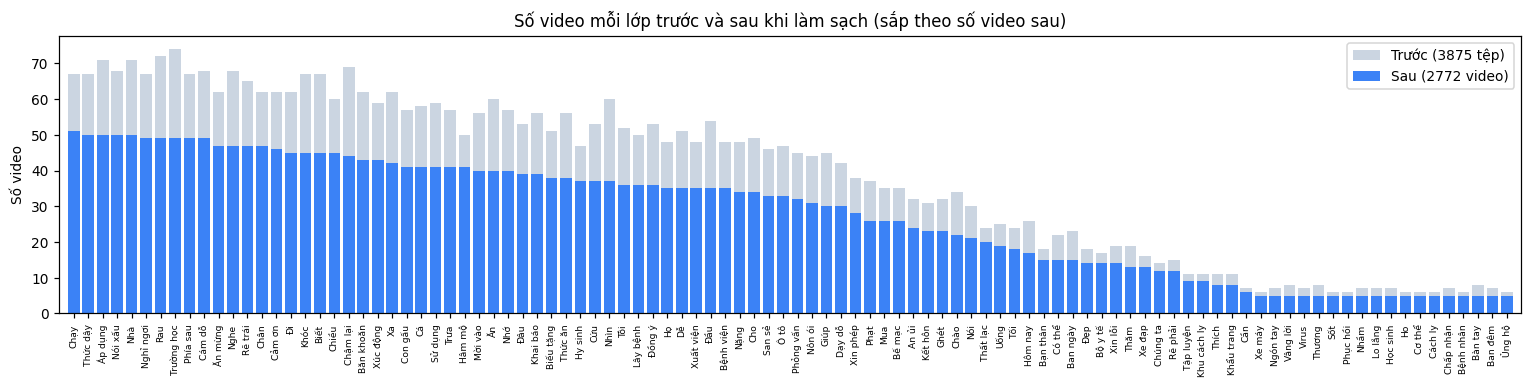
\includegraphics[width=\textwidth]{processing/class_counts_before_after.png}
  \caption{Số video mỗi lớp trước (xám) và sau (xanh) khi làm sạch, sắp xếp theo số video sau làm sạch.}
  \label{fig:pp_class_counts}
\end{figure}

% =====================================================================
\subsubsection{Xử lý khung nhiễu và lấy mẫu theo thời gian}
\label{subsec:pp_frames}

\paragraph{Bước 5 -- Đánh dấu khung đơn sắc} Gọi $f_i$ là khung thứ $i$ của video và $\sigma_c(f_i)$ là độ lệch chuẩn giá trị điểm ảnh trên kênh màu $c\in\{R,G,B\}$. Khung $f_i$ được coi là \emph{đơn sắc} nếu
\begin{equation}
  \max_{c\in\{R,G,B\}} \sigma_c(f_i) < 3,
\end{equation}
tức gần như mọi điểm ảnh có cùng một màu; ngưỡng này giống với ngưỡng ở bước EDA. Các khung còn lại là \emph{khung hợp lệ}. Thay vì xoá khung khỏi tệp video, notebook lưu danh sách chỉ số khung hợp lệ $V=(v_1<v_2<\dots<v_m)$ của từng video vào cột \texttt{valid\_idx} của manifest; khi đọc video, \texttt{preprocess.py} chỉ lấy mẫu trong danh sách này.

Trong 2.772 video sạch, 563 video (20,3\%, thuộc 78 lớp) có khung đơn sắc, trung bình 12,2 khung mỗi video. Sau khi bỏ khung đơn sắc, mỗi video còn từ 9 đến 30 khung hợp lệ (trung vị 30); 222 video còn ít hơn 16 khung hợp lệ (Hình~\ref{fig:pp_valid_hist}).

\begin{figure}[H]
  \centering
  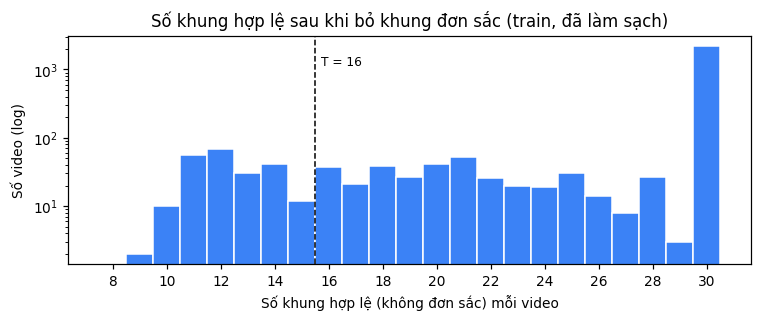
\includegraphics[width=0.75\textwidth]{processing/valid_frames_hist.png}
  \caption{Phân phối số khung hợp lệ mỗi video sau khi bỏ khung đơn sắc (trục tung thang log). Các video bên trái đường đứt nét có ít hơn $T=16$ khung hợp lệ.}
  \label{fig:pp_valid_hist}
\end{figure}

\paragraph{Bước 6 -- Lấy mẫu $T=16$ khung} Mô hình cần chuỗi đầu vào có độ dài cố định, nên mỗi video được thu gọn thành $T=16$ khung lấy đều theo thời gian trên danh sách khung hợp lệ:
\begin{equation}
  s_k = v_{\,1+\operatorname{round}\left(k\,\frac{m-1}{T-1}\right)}, \qquad k = 0, 1, \dots, T-1.
\end{equation}
Khung đầu và khung cuối của chuỗi luôn là khung hợp lệ đầu tiên và cuối cùng. Với video có $m<16$ khung hợp lệ, công thức trên tự lặp lại đều các khung (mỗi khung xuất hiện một hoặc hai lần) thay vì chỉ lặp khung cuối, nên chuỗi vẫn giữ đúng thứ tự thời gian. Nếu một video không có khung hợp lệ nào (chỉ có thể xảy ra ở dữ liệu kiểm tra hoặc demo) thì dùng toàn bộ khung.

Để thấy tác dụng của bước 5, nhóm so sánh với cách lấy mẫu đều trực tiếp trên toàn bộ khung, không lọc khung đơn sắc (Bảng~\ref{tab:pp_sampling}, Hình~\ref{fig:pp_sampling}). Nếu không lọc, cả 563 video có khung đơn sắc đều bị lẫn khung đơn sắc vào chuỗi đầu vào, trung bình 6,4/16 khung, và 222 video bị lẫn từ một nửa chuỗi trở lên; các số này khớp với mô phỏng ở bước EDA (Mục~\ref{subsec:eda_quality}). Khi lấy mẫu trên khung hợp lệ thì không còn khung đơn sắc nào trong đầu vào.

\begin{table}[H]
  \centering
  \caption{Số khung đơn sắc trong chuỗi 16 khung đầu vào, khi không lọc và khi lọc khung đơn sắc (2.772 video train sạch).}
  \label{tab:pp_sampling}
  \small
  \begin{tabular}{@{}lrr@{}}
    \toprule
    \textbf{Chỉ số} & \textbf{Không lọc} & \textbf{Có lọc} \\
    \midrule
    Video có $\geq$1 khung đơn sắc trong đầu vào   & 563 & 0 \\
    Số khung đơn sắc trung bình (trên các video đó) & 6,4/16 & 0 \\
    Video có $\geq$8/16 khung đơn sắc               & 222 & 0 \\
    \bottomrule
  \end{tabular}
\end{table}

\begin{figure}[H]
  \centering
  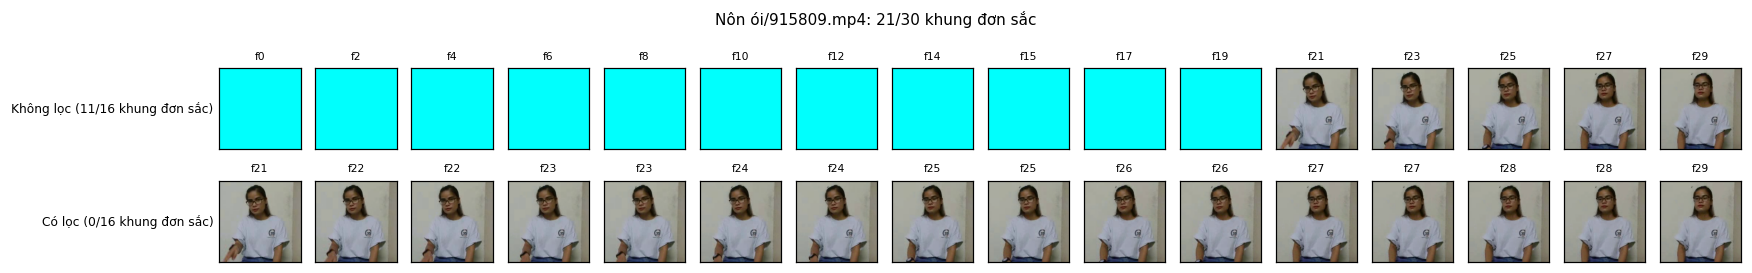
\includegraphics[width=\textwidth]{processing/sampling_naive_vs_filtered.png}
  \caption{Mười sáu khung đầu vào của video \textit{Nôn ói}/915809 (21/30 khung đơn sắc). Hàng trên: lấy mẫu trực tiếp, 11/16 khung là khung đơn sắc. Hàng dưới: lấy mẫu trên các khung hợp lệ $f_{21}$--$f_{29}$, các khung được lặp đều.}
  \label{fig:pp_sampling}
\end{figure}

% =====================================================================
\subsubsection{Chuẩn hoá}
\label{subsec:pp_norm}

\paragraph{Bước 7 -- Chuẩn hoá z-score} Giá trị điểm ảnh được đưa về $[0,1]$ rồi chuẩn hoá z-score trên từng kênh màu:
\begin{equation}
  x'_c = \frac{x_c/255 - \mu_c}{\sigma_c}, \qquad \mu = (0{,}485;\ 0{,}456;\ 0{,}406), \quad \sigma = (0{,}229;\ 0{,}224;\ 0{,}225),
\end{equation}
với $\mu,\sigma$ là trung bình và độ lệch chuẩn của tập ImageNet. Nhóm dùng thống kê của ImageNet thay vì tính lại trên tập train vì các mô hình ở Chương~\ref{sec:model} dùng mạng trích đặc trưng đã huấn luyện sẵn trên ImageNet; đầu vào cần có cùng phân phối với dữ liệu mà mạng đó đã học. Kết quả của mỗi video là một tensor kích thước $16\times3\times224\times224$. Độ phân giải đã đồng nhất $224\times224$ (Bảng~\ref{tab:eda_res}) nên không cần đổi kích thước.

% =====================================================================
\subsubsection{Chia tập huấn luyện và kiểm định}
\label{subsec:pp_split}

\paragraph{Bước 8 -- Chia phân tầng} Chỉ tập train có nhãn, nên tập kiểm định (\textit{validation}) phải tách ra từ chính tập này. Nhóm chia 2.772 video sạch thành 5 phần bằng \texttt{StratifiedKFold} của scikit-learn~\cite{sklearn} (\texttt{shuffle=True}, \texttt{random\_state=42}) và ghi số thứ tự phần vào cột \texttt{fold} của manifest. Phần \texttt{fold = 0} là tập kiểm định chung cho \emph{mọi} mô hình, các phần còn lại là tập huấn luyện; nhờ vậy kết quả của các mô hình so sánh được với nhau. Mô hình SVM có thể dùng cả 5 phần để kiểm định chéo (\textit{cross-validation}).

\begin{itemize}
  \item \textbf{Phân tầng theo nhãn:} mỗi phần giữ tỷ lệ các lớp gần giống toàn tập. Lớp nhỏ nhất có 5 video nên có đúng 1 video ở mỗi phần, nhờ đó cả 100 lớp đều có mặt ở tập kiểm định.
  \item \textbf{Không rò rỉ dữ liệu:} EDA khuyến nghị chia theo nhóm video gốc (\texttt{StratifiedGroupKFold}) để các bản sao không rơi vào cả hai phía. Vì bước 2 đã loại mọi bản sao, mỗi video sạch là một nhóm riêng, nên chia theo từng video cũng chính là chia theo nhóm. Notebook kiểm tra lại bằng \texttt{assert}: mã MD5 là duy nhất trong manifest và không có mã MD5 nào nằm ở cả tập huấn luyện lẫn tập kiểm định. Nhóm đã thử \texttt{StratifiedGroupKFold}, nhưng thuật toán này chỉ cân bằng gần đúng và tạo ra phần thiếu lớp.
\end{itemize}

\begin{table}[H]
  \centering
  \caption{Kết quả chia tập train sạch.}
  \label{tab:pp_split}
  \small
  \begin{tabular}{@{}lrrr@{}}
    \toprule
    \textbf{Tập} & \textbf{Số video} & \textbf{Số lớp} & \textbf{Số video mỗi lớp} \\
    \midrule
    Huấn luyện (\texttt{fold} 1--4) & 2.217 & 100 & 4--41 \\
    Kiểm định (\texttt{fold} 0)     & 555   & 100 & 1--10 \\
    \midrule
    Tổng                            & 2.772 & 100 & 5--51 \\
    \bottomrule
  \end{tabular}
\end{table}

% =====================================================================
\subsubsection{Xử lý mất cân bằng lớp}
\label{subsec:pp_weights}

\paragraph{Bước 9 -- Trọng số lớp} Trên tập huấn luyện, lớp nhiều nhất (\textit{Chạy}) có 41 video còn nhiều lớp chỉ có 4 video (\textit{Cách ly}, \textit{Ho}, \textit{Sốt}, \textit{Virus}, \textit{Xe máy},\ldots), chênh khoảng 10,2 lần. Nếu mọi mẫu có vai trò như nhau trong hàm mất mát, mô hình sẽ ưu tiên các lớp đông và Macro F1 giảm ở các lớp ít mẫu. Nhóm tính trọng số cho từng lớp $c$ theo kiểu \textit{balanced}:
\begin{equation}
  w_c = \frac{N}{K \cdot n_c},
\end{equation}
với $N=2.217$ là số video huấn luyện, $K=100$ là số lớp và $n_c$ là số video huấn luyện của lớp $c$. Lớp ít mẫu nhận trọng số lớn: trọng số dao động từ 0,54 (\textit{Chạy}) đến 5,54 (các lớp có 4 video), và một lớp trung bình ($n_c = N/K$) có trọng số bằng 1. Trọng số chỉ tính trên tập huấn luyện để không dùng thông tin của tập kiểm định. Các mô hình dùng trọng số này trong hàm mất mát (ví dụ tham số \texttt{weight} của \texttt{CrossEntropyLoss}) hoặc tham số \texttt{class\_weight} của SVM.

% =====================================================================
\subsubsection{Tăng cường dữ liệu}
\label{subsec:pp_aug}

\paragraph{Bước 10 -- Tăng cường} Tập huấn luyện nhỏ (trung bình khoảng 22 video mỗi lớp), nên mỗi lần đọc một video huấn luyện, \texttt{preprocess.py} tạo ra một biến thể ngẫu nhiên khác của video đó. Ba phép biến đổi được dùng, với cùng một tham số cho mọi khung của một video để chuyển động không bị méo:

\begin{itemize}
  \item \textbf{Cắt đoạn theo thời gian:} giữ một đoạn liên tục dài 80--100\% danh sách khung hợp lệ ở vị trí ngẫu nhiên, rồi mới lấy 16 khung. Phép này mô phỏng việc người ký bắt đầu, kết thúc sớm hay muộn và ký nhanh hay chậm khác nhau.
  \item \textbf{Cắt vùng ảnh ngẫu nhiên:} cắt một vùng có cạnh bằng 85--100\% cạnh khung hình ở vị trí ngẫu nhiên rồi phóng lại về $224\times224$. Phép này mô phỏng khác biệt về vị trí người ký và khoảng cách tới máy quay.
  \item \textbf{Thay đổi màu:} nhân độ sáng, độ tương phản và độ bão hoà với các hệ số ngẫu nhiên trong khoảng $[0{,}75;\ 1{,}25]$, giúp mô hình bền vững với khác biệt ánh sáng và màu nền giữa train và test (Mục~\ref{subsec:eda_shift}).
\end{itemize}

Nhóm \emph{không} dùng lật ngang vì tay trái và tay phải có thể làm đổi nghĩa ký hiệu. Tăng cường chỉ áp dụng cho tập huấn luyện; tập kiểm định và tập kiểm tra được đưa vào mô hình nguyên bản để kết quả đánh giá ổn định. Hình~\ref{fig:pp_aug} minh hoạ ba biến thể tạo ra từ cùng một video.

\begin{figure}[H]
  \centering
  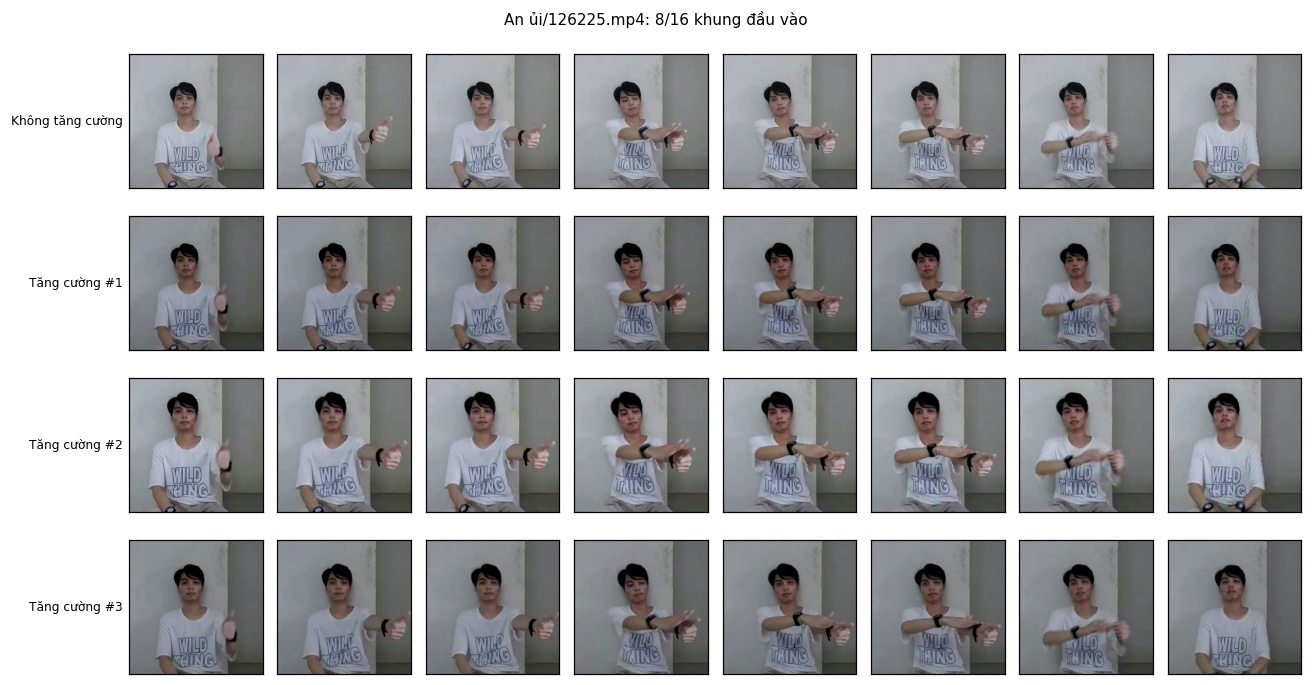
\includegraphics[width=0.9\textwidth]{processing/augmentation_examples.png}
  \caption{Một video lớp \textit{An ủi} (hàng đầu) và ba biến thể tăng cường ngẫu nhiên; mỗi hàng hiển thị 8 trong 16 khung đầu vào.}
  \label{fig:pp_aug}
\end{figure}

% =====================================================================
\subsubsection{Dữ liệu kiểm tra}
\label{subsec:pp_test}

Hai tập kiểm tra (\texttt{public\_test}, \texttt{private\_test}) không có nhãn và cuộc thi yêu cầu dự đoán cho \emph{mọi} tệp, nên nhóm không loại tệp nào. Notebook chỉ lập bảng \texttt{test\_manifest.csv} gồm tên tệp, mã MD5 và cột \texttt{dup\_of\_train} đánh dấu video trùng với tập train: có 157/1.630 video public test trùng với train và 0/2.859 video private test trùng với train. Các video trùng vẫn được mô hình dự đoán bình thường; cột này chỉ dùng khi diễn giải điểm public test (Mục~\ref{subsec:eda_quality}).

Khi suy luận, mỗi video kiểm tra đi qua đúng các bước 5, 6 và 7 như video kiểm định: tự tìm khung đơn sắc, lấy 16 khung trên các khung hợp lệ và chuẩn hoá, không tăng cường. Notebook chạy thử hàm đọc video này trên 8 video kiểm tra ngẫu nhiên để xác nhận đầu ra có đúng kích thước $16\times224\times224\times3$.

% =====================================================================
\subsubsection{Kết quả và đầu ra}
\label{subsec:pp_output}

Bảng~\ref{tab:pp_outputs} liệt kê các tệp do notebook tạo ra trong thư mục \texttt{processing/output/}. Các mô hình chỉ cần \texttt{preprocess.py}, \texttt{manifest\_clean.csv}, \texttt{test\_manifest.csv} và \texttt{class\_weights.csv} (vài trăm KB) cùng tệp dữ liệu gốc, không cần chạy lại bước làm sạch.

\begin{table}[H]
  \centering
  \caption{Các tệp đầu ra của bước tiền xử lý.}
  \label{tab:pp_outputs}
  \small
  \begin{tabular}{@{}p{0.3\textwidth}p{0.62\textwidth}@{}}
    \toprule
    \textbf{Tệp} & \textbf{Nội dung} \\
    \midrule
    \texttt{manifest\_clean.csv} & 2.772 video train sạch: lớp, nhãn số, tên tệp, đường dẫn, MD5, số khung, số khung hợp lệ, chỉ số khung hợp lệ (\texttt{valid\_idx}), phần (\texttt{fold}) \\
    \texttt{removed.csv} & 1.103 tệp bị loại, kèm bước và lý do \\
    \texttt{test\_manifest.csv} & 4.489 video kiểm tra: tập, tên tệp, MD5, \texttt{dup\_of\_train} \\
    \texttt{class\_weights.csv} & Trọng số 100 lớp tính trên tập huấn luyện \\
    \texttt{processing\_summary.csv} & Số video còn lại sau từng bước (Bảng~\ref{tab:pp_flow}) \\
    \texttt{class\_counts\_before\_after.csv} & Số video mỗi lớp trước và sau làm sạch \\
    \texttt{processing\_config.json} & Tham số đã dùng (\texttt{SEED}, số phần, $T$, ngưỡng đơn sắc) \\
    \texttt{figures/} & Các hình trong mục này \\
    \bottomrule
  \end{tabular}
\end{table}

Tóm lại, sau tiền xử lý tập train không còn bản sao, video rỗng hay nhãn mâu thuẫn; không video nào còn khung đơn sắc trong chuỗi đầu vào; tập kiểm định đủ 100 lớp và không chứa video trùng với tập huấn luyện. Các bước này xử lý cả ba vấn đề chính mà EDA đã nêu: bản sao gây rò rỉ dữ liệu, khung đơn sắc chỉ có ở train và mất cân bằng lớp.

\paragraph{Hạn chế} Nhóm chưa xác định được nhãn đúng cho hai nội dung xung đột nên phải bỏ chúng, làm giảm 5 tệp dữ liệu có thể hữu ích. Ngưỡng đơn sắc chỉ phát hiện khung một màu hoàn toàn, chưa phát hiện khung mờ hoặc khung chỉ có nền. Khử trùng lặp bằng MD5 chỉ tìm được bản sao giống hệt từng byte, không tìm được video gần giống nhau (ví dụ cùng cảnh nhưng nén lại). Cuối cùng, tập kiểm định chỉ có 1--10 video mỗi lớp, nên F1 của từng lớp riêng lẻ trên tập này còn dao động lớn.
]
% Mã nguồn: processing/data_processing.ipynb, processing/preprocess.py
% Hình: image/processing/*.png (sinh từ processing/output/figures/)
%   3.2.1 Tổng quan quy trình
%   3.2.2 Làm sạch dữ liệu
%   3.2.3 Xử lý khung nhiễu và lấy mẫu theo thời gian
%   3.2.4 Chuẩn hoá
%   3.2.5 Chia tập huấn luyện và kiểm định
%   3.2.6 Xử lý mất cân bằng lớp
%   3.2.7 Tăng cường dữ liệu
%   3.2.8 Dữ liệu kiểm tra
%   3.2.9 Kết quả và đầu ra
% =====================================================================

\subsection{Tiền xử lý dữ liệu}
\label{sec:preprocess}

Mục này trình bày các bước biến dữ liệu thô thành đầu vào sạch và thống nhất cho mọi mô hình ở Chương~\ref{sec:model}. Mỗi bước xuất phát từ một vấn đề đã phát hiện ở bước EDA (Bảng~\ref{tab:eda_reco}). Nhóm dùng Python với \texttt{pandas}, \texttt{numpy}, \texttt{OpenCV} và \texttt{scikit-learn}; mã nguồn gồm hai phần:

\begin{itemize}
  \item \textbf{Notebook làm sạch} \texttt{processing/data\_processing.ipynb}: chạy \emph{một lần} trên toàn bộ tập train để kiểm tra, loại bỏ và đánh dấu dữ liệu lỗi, chia tập kiểm định và tính trọng số lớp. Kết quả được lưu thành một bảng chỉ mục (\textit{manifest}) dùng chung cho cả nhóm.
  \item \textbf{Module dùng chung} \texttt{processing/preprocess.py}: các phép biến đổi áp dụng \emph{mỗi lần} mô hình đọc một video (bỏ khung đơn sắc, lấy mẫu khung, tăng cường, chuẩn hoá). Mô hình SVM, CNN-LSTM, Vision Transformer và ứng dụng demo cùng gọi module này, nên dữ liệu ở huấn luyện, kiểm định, kiểm tra và demo được xử lý giống hệt nhau.
\end{itemize}

Nhóm không lưu sẵn khung hình đã xử lý ra đĩa vì hai lý do: lưu 16 khung $224\times224\times3$ cho 2.772 video tốn khoảng 6,7~GB, và phép tăng cường cần tạo ra phiên bản khác nhau ở mỗi lần đọc. Mọi bước có yếu tố ngẫu nhiên đều cố định hạt giống \texttt{SEED = 42} để kết quả tái lập được.

% =====================================================================
\subsubsection{Tổng quan quy trình}
\label{subsec:pp_overview}

Bảng~\ref{tab:pp_overview} liệt kê mười bước tiền xử lý theo thứ tự thực hiện và xếp mỗi bước vào nhóm tác vụ tiền xử lý dữ liệu tương ứng: làm sạch (\textit{data cleaning}), tích hợp (\textit{data integration}), thu gọn (\textit{data reduction}) và biến đổi dữ liệu (\textit{data transformation})~\cite{han2011}.

\begin{table}[H]
  \centering
  \caption{Các bước tiền xử lý, nhóm tác vụ và nơi thực hiện.}
  \label{tab:pp_overview}
  \small
  \begin{tabular}{@{}cp{0.33\textwidth}p{0.3\textwidth}p{0.2\textwidth}@{}}
    \toprule
    \textbf{Bước} & \textbf{Việc} & \textbf{Nhóm tác vụ} & \textbf{Thực hiện ở} \\
    \midrule
    1  & Kiểm tra toàn vẹn, chuẩn hoá tên lớp & Làm sạch: dữ liệu thiếu, lỗi & Notebook \\
    2  & Khử trùng lặp theo MD5 & Tích hợp: dư thừa dữ liệu & Notebook \\
    3  & Loại video xung đột nhãn & Làm sạch: dữ liệu không nhất quán & Notebook \\
    4  & Loại video rỗng & Làm sạch: dữ liệu thiếu & Notebook \\
    5  & Đánh dấu khung đơn sắc & Làm sạch: dữ liệu nhiễu & Notebook, \texttt{preprocess.py} \\
    6  & Lấy đều $T=16$ khung trên các khung hợp lệ & Thu gọn: lấy mẫu & \texttt{preprocess.py} \\
    7  & Chuẩn hoá z-score theo kênh màu & Biến đổi: chuẩn hoá & \texttt{preprocess.py} \\
    8  & Chia train/validation phân tầng & Đánh giá mô hình & Notebook \\
    9  & Trọng số lớp & Xử lý mất cân bằng lớp & Notebook \\
    10 & Tăng cường dữ liệu (chỉ khi huấn luyện) & Sinh thêm dữ liệu & \texttt{preprocess.py} \\
    \bottomrule
  \end{tabular}
\end{table}

Bước 1--5 thu hẹp tập train từ 3.875 tệp xuống 2.772 video sạch (Bảng~\ref{tab:pp_flow}). Bước 6, 7 và 10 không bỏ video nào mà quyết định video được đưa vào mô hình dưới dạng nào. Bước 8 và 9 chuẩn bị cho huấn luyện và đánh giá.

% =====================================================================
\subsubsection{Làm sạch dữ liệu}
\label{subsec:pp_clean}

\paragraph{Quét toàn bộ video} Notebook mở từng video bằng \texttt{cv2.VideoCapture}, đọc \emph{tất cả} khung hình và ghi lại: mã băm MD5 của tệp, số khung, và danh sách chỉ số các khung không đơn sắc (Mục~\ref{subsec:pp_frames}). Việc quét được chạy song song trên nhiều lõi CPU (\texttt{ProcessPoolExecutor}). Để kiểm tra bước quét, nhóm đối chiếu số khung đơn sắc của từng video với cột \texttt{solid\_frames} trong \texttt{video\_quality\_flags.csv} của bước EDA: cả 3.875/3.875 tệp đều khớp.

\paragraph{Bước 1 -- Kiểm tra toàn vẹn} Cả 3.875 tệp đều đọc được và có ít nhất 16 khung, nên không có tệp nào bị loại ở bước này. Tên lớp ở thư mục và khoá trong \texttt{label\_mapping.pkl} được chuẩn hoá về dạng Unicode NFC trước khi so khớp (Mục~\ref{subsec:eda_structure}); sau chuẩn hoá, 100/100 lớp có nhãn số 0--99.

\paragraph{Bước 2 -- Khử trùng lặp} Hai tệp có cùng mã MD5 là cùng một video. Với mỗi mã MD5, notebook giữ lại một tệp (ưu tiên tệp không có hậu tố \texttt{\_N}) và loại các tệp còn lại. Bước này loại 1.099 tệp, trong đó 1.069 tệp mang hậu tố \texttt{\_N}, và còn \textbf{2.776 video duy nhất}, khớp với kết quả EDA. Từ đây mỗi video trong tập sạch có một mã MD5 riêng; tính chất này giúp chia tập kiểm định không bị rò rỉ (Mục~\ref{subsec:pp_split}).

\paragraph{Bước 3 -- Xung đột nhãn} Hai nội dung video vừa nằm ở lớp \textit{Chào} vừa nằm ở lớp \textit{Chậm lại} (5 tệp: \texttt{Chào/392683}, \texttt{Chào/468203}, \texttt{Chào/792094}, \texttt{Chậm lại/254739}, \texttt{Chậm lại/284430}). Nhóm không xác minh được nhãn nào đúng, và giữ một video với nhãn có thể sai sẽ đưa nhiễu nhãn vào cả huấn luyện lẫn đánh giá, nên loại toàn bộ hai nội dung này. Notebook có sẵn biến \texttt{KEEP\_LABEL} để giữ lại các video này với nhãn đã xác minh nếu sau này có thông tin. Sau bước này còn 2.774 video. Hai lớp bị ảnh hưởng vẫn còn nhiều mẫu (\textit{Chào} 22 video, \textit{Chậm lại} 44 video).

\paragraph{Bước 4 -- Video rỗng} Hai video không có khung hợp lệ nào (\texttt{Biết/214576}: 16/16 khung đơn sắc; \texttt{Khai báo/885339}: 23/23 khung đơn sắc) bị loại vì không chứa thông tin ký hiệu. Tập train sạch còn \textbf{2.772 video} và vẫn đủ 100 lớp.

\begin{table}[H]
  \centering
  \caption{Số video còn lại sau từng bước làm sạch tập train.}
  \label{tab:pp_flow}
  \small
  \begin{tabular}{@{}p{0.3\textwidth}rp{0.45\textwidth}@{}}
    \toprule
    \textbf{Bước} & \textbf{Còn lại} & \textbf{Ghi chú} \\
    \midrule
    Ban đầu                          & 3.875 & Toàn bộ tệp trong \texttt{train/} \\
    1 -- Kiểm tra toàn vẹn           & 3.875 & Không có tệp lỗi hoặc thiếu khung \\
    2 -- Khử trùng lặp MD5           & 2.776 & Loại 1.099 bản sao \\
    3 -- Xung đột nhãn               & 2.774 & Loại 2 nội dung (5 tệp) \textit{Chào} $\leftrightarrow$ \textit{Chậm lại} \\
    4 -- Video rỗng                  & \textbf{2.772} & Loại \texttt{Biết/214576}, \texttt{Khai báo/885339} \\
    5 -- Khung đơn sắc               & 2.772 & 563 video có khung bị bỏ qua, không loại video \\
    \bottomrule
  \end{tabular}
\end{table}

Danh sách 1.103 tệp bị loại cùng lý do được lưu ở \texttt{processing/output/removed.csv}, để có thể kiểm tra lại từng trường hợp. Hình~\ref{fig:pp_class_counts} so sánh số video mỗi lớp trước và sau khi làm sạch: sau làm sạch mỗi lớp có từ 5 đến 51 video (trung bình 27,7; trung vị 32,5).

\begin{figure}[H]
  \centering
  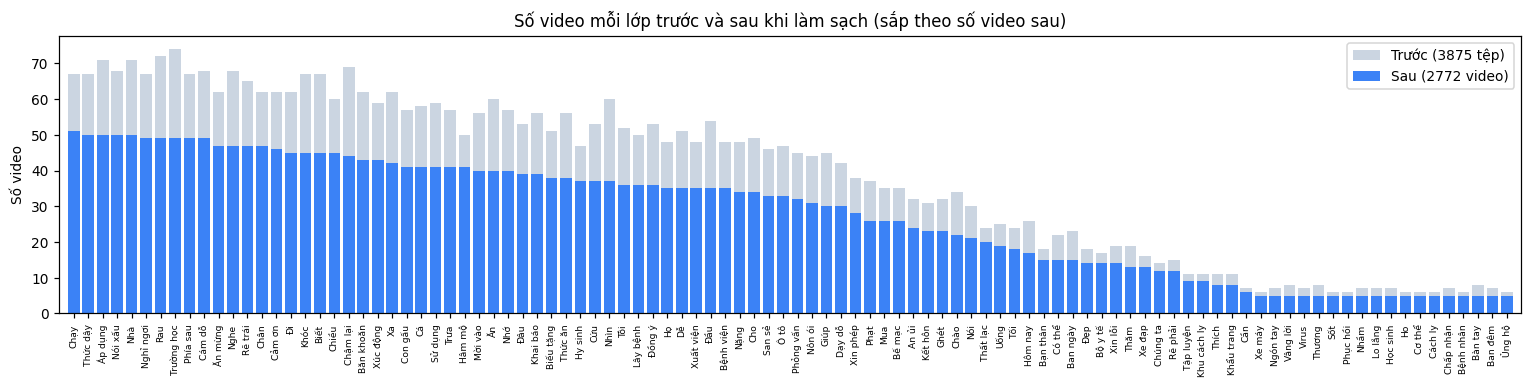
\includegraphics[width=\textwidth]{processing/class_counts_before_after.png}
  \caption{Số video mỗi lớp trước (xám) và sau (xanh) khi làm sạch, sắp xếp theo số video sau làm sạch.}
  \label{fig:pp_class_counts}
\end{figure}

% =====================================================================
\subsubsection{Xử lý khung nhiễu và lấy mẫu theo thời gian}
\label{subsec:pp_frames}

\paragraph{Bước 5 -- Đánh dấu khung đơn sắc} Gọi $f_i$ là khung thứ $i$ của video và $\sigma_c(f_i)$ là độ lệch chuẩn giá trị điểm ảnh trên kênh màu $c\in\{R,G,B\}$. Khung $f_i$ được coi là \emph{đơn sắc} nếu
\begin{equation}
  \max_{c\in\{R,G,B\}} \sigma_c(f_i) < 3,
\end{equation}
tức gần như mọi điểm ảnh có cùng một màu; ngưỡng này giống với ngưỡng ở bước EDA. Các khung còn lại là \emph{khung hợp lệ}. Thay vì xoá khung khỏi tệp video, notebook lưu danh sách chỉ số khung hợp lệ $V=(v_1<v_2<\dots<v_m)$ của từng video vào cột \texttt{valid\_idx} của manifest; khi đọc video, \texttt{preprocess.py} chỉ lấy mẫu trong danh sách này.

Trong 2.772 video sạch, 563 video (20,3\%, thuộc 78 lớp) có khung đơn sắc, trung bình 12,2 khung mỗi video. Sau khi bỏ khung đơn sắc, mỗi video còn từ 9 đến 30 khung hợp lệ (trung vị 30); 222 video còn ít hơn 16 khung hợp lệ (Hình~\ref{fig:pp_valid_hist}).

\begin{figure}[H]
  \centering
  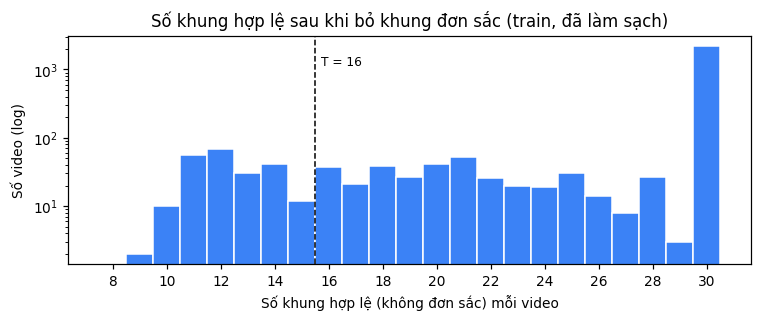
\includegraphics[width=0.75\textwidth]{processing/valid_frames_hist.png}
  \caption{Phân phối số khung hợp lệ mỗi video sau khi bỏ khung đơn sắc (trục tung thang log). Các video bên trái đường đứt nét có ít hơn $T=16$ khung hợp lệ.}
  \label{fig:pp_valid_hist}
\end{figure}

\paragraph{Bước 6 -- Lấy mẫu $T=16$ khung} Mô hình cần chuỗi đầu vào có độ dài cố định, nên mỗi video được thu gọn thành $T=16$ khung lấy đều theo thời gian trên danh sách khung hợp lệ:
\begin{equation}
  s_k = v_{\,1+\operatorname{round}\left(k\,\frac{m-1}{T-1}\right)}, \qquad k = 0, 1, \dots, T-1.
\end{equation}
Khung đầu và khung cuối của chuỗi luôn là khung hợp lệ đầu tiên và cuối cùng. Với video có $m<16$ khung hợp lệ, công thức trên tự lặp lại đều các khung (mỗi khung xuất hiện một hoặc hai lần) thay vì chỉ lặp khung cuối, nên chuỗi vẫn giữ đúng thứ tự thời gian. Nếu một video không có khung hợp lệ nào (chỉ có thể xảy ra ở dữ liệu kiểm tra hoặc demo) thì dùng toàn bộ khung.

Để thấy tác dụng của bước 5, nhóm so sánh với cách lấy mẫu đều trực tiếp trên toàn bộ khung, không lọc khung đơn sắc (Bảng~\ref{tab:pp_sampling}, Hình~\ref{fig:pp_sampling}). Nếu không lọc, cả 563 video có khung đơn sắc đều bị lẫn khung đơn sắc vào chuỗi đầu vào, trung bình 6,4/16 khung, và 222 video bị lẫn từ một nửa chuỗi trở lên; các số này khớp với mô phỏng ở bước EDA (Mục~\ref{subsec:eda_quality}). Khi lấy mẫu trên khung hợp lệ thì không còn khung đơn sắc nào trong đầu vào.

\begin{table}[H]
  \centering
  \caption{Số khung đơn sắc trong chuỗi 16 khung đầu vào, khi không lọc và khi lọc khung đơn sắc (2.772 video train sạch).}
  \label{tab:pp_sampling}
  \small
  \begin{tabular}{@{}lrr@{}}
    \toprule
    \textbf{Chỉ số} & \textbf{Không lọc} & \textbf{Có lọc} \\
    \midrule
    Video có $\geq$1 khung đơn sắc trong đầu vào   & 563 & 0 \\
    Số khung đơn sắc trung bình (trên các video đó) & 6,4/16 & 0 \\
    Video có $\geq$8/16 khung đơn sắc               & 222 & 0 \\
    \bottomrule
  \end{tabular}
\end{table}

\begin{figure}[H]
  \centering
  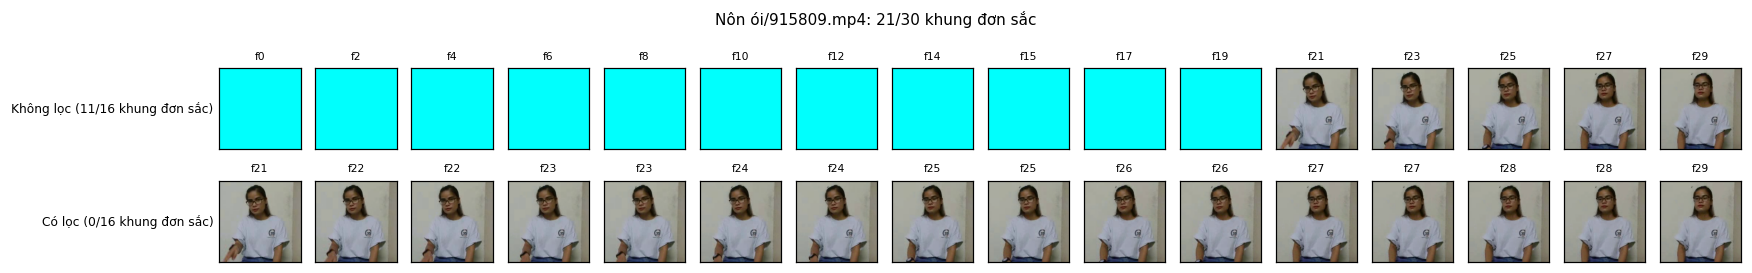
\includegraphics[width=\textwidth]{processing/sampling_naive_vs_filtered.png}
  \caption{Mười sáu khung đầu vào của video \textit{Nôn ói}/915809 (21/30 khung đơn sắc). Hàng trên: lấy mẫu trực tiếp, 11/16 khung là khung đơn sắc. Hàng dưới: lấy mẫu trên các khung hợp lệ $f_{21}$--$f_{29}$, các khung được lặp đều.}
  \label{fig:pp_sampling}
\end{figure}

% =====================================================================
\subsubsection{Chuẩn hoá}
\label{subsec:pp_norm}

\paragraph{Bước 7 -- Chuẩn hoá z-score} Giá trị điểm ảnh được đưa về $[0,1]$ rồi chuẩn hoá z-score trên từng kênh màu:
\begin{equation}
  x'_c = \frac{x_c/255 - \mu_c}{\sigma_c}, \qquad \mu = (0{,}485;\ 0{,}456;\ 0{,}406), \quad \sigma = (0{,}229;\ 0{,}224;\ 0{,}225),
\end{equation}
với $\mu,\sigma$ là trung bình và độ lệch chuẩn của tập ImageNet. Nhóm dùng thống kê của ImageNet thay vì tính lại trên tập train vì các mô hình ở Chương~\ref{sec:model} dùng mạng trích đặc trưng đã huấn luyện sẵn trên ImageNet; đầu vào cần có cùng phân phối với dữ liệu mà mạng đó đã học. Kết quả của mỗi video là một tensor kích thước $16\times3\times224\times224$. Độ phân giải đã đồng nhất $224\times224$ (Bảng~\ref{tab:eda_res}) nên không cần đổi kích thước.

% =====================================================================
\subsubsection{Chia tập huấn luyện và kiểm định}
\label{subsec:pp_split}

\paragraph{Bước 8 -- Chia phân tầng} Chỉ tập train có nhãn, nên tập kiểm định (\textit{validation}) phải tách ra từ chính tập này. Nhóm chia 2.772 video sạch thành 5 phần bằng \texttt{StratifiedKFold} của scikit-learn~\cite{sklearn} (\texttt{shuffle=True}, \texttt{random\_state=42}) và ghi số thứ tự phần vào cột \texttt{fold} của manifest. Phần \texttt{fold = 0} là tập kiểm định chung cho \emph{mọi} mô hình, các phần còn lại là tập huấn luyện; nhờ vậy kết quả của các mô hình so sánh được với nhau. Mô hình SVM có thể dùng cả 5 phần để kiểm định chéo (\textit{cross-validation}).

\begin{itemize}
  \item \textbf{Phân tầng theo nhãn:} mỗi phần giữ tỷ lệ các lớp gần giống toàn tập. Lớp nhỏ nhất có 5 video nên có đúng 1 video ở mỗi phần, nhờ đó cả 100 lớp đều có mặt ở tập kiểm định.
  \item \textbf{Không rò rỉ dữ liệu:} EDA khuyến nghị chia theo nhóm video gốc (\texttt{StratifiedGroupKFold}) để các bản sao không rơi vào cả hai phía. Vì bước 2 đã loại mọi bản sao, mỗi video sạch là một nhóm riêng, nên chia theo từng video cũng chính là chia theo nhóm. Notebook kiểm tra lại bằng \texttt{assert}: mã MD5 là duy nhất trong manifest và không có mã MD5 nào nằm ở cả tập huấn luyện lẫn tập kiểm định. Nhóm đã thử \texttt{StratifiedGroupKFold}, nhưng thuật toán này chỉ cân bằng gần đúng và tạo ra phần thiếu lớp.
\end{itemize}

\begin{table}[H]
  \centering
  \caption{Kết quả chia tập train sạch.}
  \label{tab:pp_split}
  \small
  \begin{tabular}{@{}lrrr@{}}
    \toprule
    \textbf{Tập} & \textbf{Số video} & \textbf{Số lớp} & \textbf{Số video mỗi lớp} \\
    \midrule
    Huấn luyện (\texttt{fold} 1--4) & 2.217 & 100 & 4--41 \\
    Kiểm định (\texttt{fold} 0)     & 555   & 100 & 1--10 \\
    \midrule
    Tổng                            & 2.772 & 100 & 5--51 \\
    \bottomrule
  \end{tabular}
\end{table}

% =====================================================================
\subsubsection{Xử lý mất cân bằng lớp}
\label{subsec:pp_weights}

\paragraph{Bước 9 -- Trọng số lớp} Trên tập huấn luyện, lớp nhiều nhất (\textit{Chạy}) có 41 video còn nhiều lớp chỉ có 4 video (\textit{Cách ly}, \textit{Ho}, \textit{Sốt}, \textit{Virus}, \textit{Xe máy},\ldots), chênh khoảng 10,2 lần. Nếu mọi mẫu có vai trò như nhau trong hàm mất mát, mô hình sẽ ưu tiên các lớp đông và Macro F1 giảm ở các lớp ít mẫu. Nhóm tính trọng số cho từng lớp $c$ theo kiểu \textit{balanced}:
\begin{equation}
  w_c = \frac{N}{K \cdot n_c},
\end{equation}
với $N=2.217$ là số video huấn luyện, $K=100$ là số lớp và $n_c$ là số video huấn luyện của lớp $c$. Lớp ít mẫu nhận trọng số lớn: trọng số dao động từ 0,54 (\textit{Chạy}) đến 5,54 (các lớp có 4 video), và một lớp trung bình ($n_c = N/K$) có trọng số bằng 1. Trọng số chỉ tính trên tập huấn luyện để không dùng thông tin của tập kiểm định. Các mô hình dùng trọng số này trong hàm mất mát (ví dụ tham số \texttt{weight} của \texttt{CrossEntropyLoss}) hoặc tham số \texttt{class\_weight} của SVM.

% =====================================================================
\subsubsection{Tăng cường dữ liệu}
\label{subsec:pp_aug}

\paragraph{Bước 10 -- Tăng cường} Tập huấn luyện nhỏ (trung bình khoảng 22 video mỗi lớp), nên mỗi lần đọc một video huấn luyện, \texttt{preprocess.py} tạo ra một biến thể ngẫu nhiên khác của video đó. Ba phép biến đổi được dùng, với cùng một tham số cho mọi khung của một video để chuyển động không bị méo:

\begin{itemize}
  \item \textbf{Cắt đoạn theo thời gian:} giữ một đoạn liên tục dài 80--100\% danh sách khung hợp lệ ở vị trí ngẫu nhiên, rồi mới lấy 16 khung. Phép này mô phỏng việc người ký bắt đầu, kết thúc sớm hay muộn và ký nhanh hay chậm khác nhau.
  \item \textbf{Cắt vùng ảnh ngẫu nhiên:} cắt một vùng có cạnh bằng 85--100\% cạnh khung hình ở vị trí ngẫu nhiên rồi phóng lại về $224\times224$. Phép này mô phỏng khác biệt về vị trí người ký và khoảng cách tới máy quay.
  \item \textbf{Thay đổi màu:} nhân độ sáng, độ tương phản và độ bão hoà với các hệ số ngẫu nhiên trong khoảng $[0{,}75;\ 1{,}25]$, giúp mô hình bền vững với khác biệt ánh sáng và màu nền giữa train và test (Mục~\ref{subsec:eda_shift}).
\end{itemize}

Nhóm \emph{không} dùng lật ngang vì tay trái và tay phải có thể làm đổi nghĩa ký hiệu. Tăng cường chỉ áp dụng cho tập huấn luyện; tập kiểm định và tập kiểm tra được đưa vào mô hình nguyên bản để kết quả đánh giá ổn định. Hình~\ref{fig:pp_aug} minh hoạ ba biến thể tạo ra từ cùng một video.

\begin{figure}[H]
  \centering
  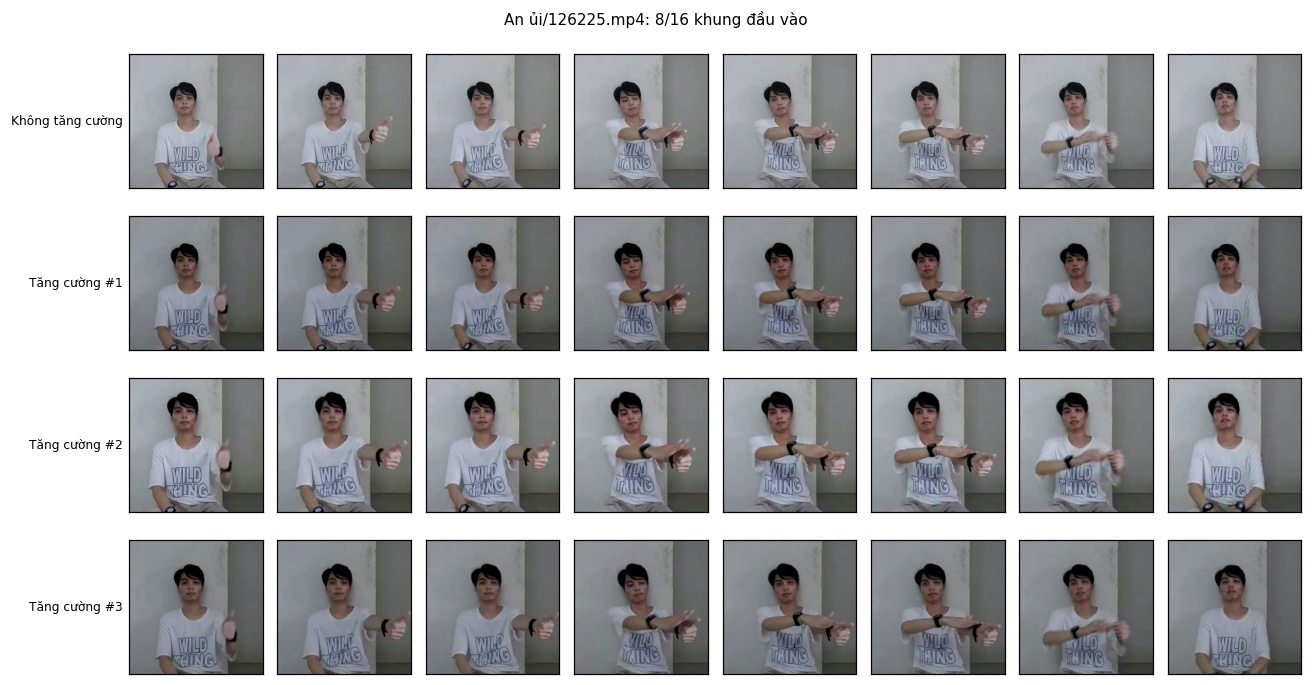
\includegraphics[width=0.9\textwidth]{processing/augmentation_examples.png}
  \caption{Một video lớp \textit{An ủi} (hàng đầu) và ba biến thể tăng cường ngẫu nhiên; mỗi hàng hiển thị 8 trong 16 khung đầu vào.}
  \label{fig:pp_aug}
\end{figure}

% =====================================================================
\subsubsection{Dữ liệu kiểm tra}
\label{subsec:pp_test}

Hai tập kiểm tra (\texttt{public\_test}, \texttt{private\_test}) không có nhãn và cuộc thi yêu cầu dự đoán cho \emph{mọi} tệp, nên nhóm không loại tệp nào. Notebook chỉ lập bảng \texttt{test\_manifest.csv} gồm tên tệp, mã MD5 và cột \texttt{dup\_of\_train} đánh dấu video trùng với tập train: có 157/1.630 video public test trùng với train và 0/2.859 video private test trùng với train. Các video trùng vẫn được mô hình dự đoán bình thường; cột này chỉ dùng khi diễn giải điểm public test (Mục~\ref{subsec:eda_quality}).

Khi suy luận, mỗi video kiểm tra đi qua đúng các bước 5, 6 và 7 như video kiểm định: tự tìm khung đơn sắc, lấy 16 khung trên các khung hợp lệ và chuẩn hoá, không tăng cường. Notebook chạy thử hàm đọc video này trên 8 video kiểm tra ngẫu nhiên để xác nhận đầu ra có đúng kích thước $16\times224\times224\times3$.

% =====================================================================
\subsubsection{Kết quả và đầu ra}
\label{subsec:pp_output}

Bảng~\ref{tab:pp_outputs} liệt kê các tệp do notebook tạo ra trong thư mục \texttt{processing/output/}. Các mô hình chỉ cần \texttt{preprocess.py}, \texttt{manifest\_clean.csv}, \texttt{test\_manifest.csv} và \texttt{class\_weights.csv} (vài trăm KB) cùng tệp dữ liệu gốc, không cần chạy lại bước làm sạch.

\begin{table}[H]
  \centering
  \caption{Các tệp đầu ra của bước tiền xử lý.}
  \label{tab:pp_outputs}
  \small
  \begin{tabular}{@{}p{0.3\textwidth}p{0.62\textwidth}@{}}
    \toprule
    \textbf{Tệp} & \textbf{Nội dung} \\
    \midrule
    \texttt{manifest\_clean.csv} & 2.772 video train sạch: lớp, nhãn số, tên tệp, đường dẫn, MD5, số khung, số khung hợp lệ, chỉ số khung hợp lệ (\texttt{valid\_idx}), phần (\texttt{fold}) \\
    \texttt{removed.csv} & 1.103 tệp bị loại, kèm bước và lý do \\
    \texttt{test\_manifest.csv} & 4.489 video kiểm tra: tập, tên tệp, MD5, \texttt{dup\_of\_train} \\
    \texttt{class\_weights.csv} & Trọng số 100 lớp tính trên tập huấn luyện \\
    \texttt{processing\_summary.csv} & Số video còn lại sau từng bước (Bảng~\ref{tab:pp_flow}) \\
    \texttt{class\_counts\_before\_after.csv} & Số video mỗi lớp trước và sau làm sạch \\
    \texttt{processing\_config.json} & Tham số đã dùng (\texttt{SEED}, số phần, $T$, ngưỡng đơn sắc) \\
    \texttt{figures/} & Các hình trong mục này \\
    \bottomrule
  \end{tabular}
\end{table}

Tóm lại, sau tiền xử lý tập train không còn bản sao, video rỗng hay nhãn mâu thuẫn; không video nào còn khung đơn sắc trong chuỗi đầu vào; tập kiểm định đủ 100 lớp và không chứa video trùng với tập huấn luyện. Các bước này xử lý cả ba vấn đề chính mà EDA đã nêu: bản sao gây rò rỉ dữ liệu, khung đơn sắc chỉ có ở train và mất cân bằng lớp.

\paragraph{Hạn chế} Nhóm chưa xác định được nhãn đúng cho hai nội dung xung đột nên phải bỏ chúng, làm giảm 5 tệp dữ liệu có thể hữu ích. Ngưỡng đơn sắc chỉ phát hiện khung một màu hoàn toàn, chưa phát hiện khung mờ hoặc khung chỉ có nền. Khử trùng lặp bằng MD5 chỉ tìm được bản sao giống hệt từng byte, không tìm được video gần giống nhau (ví dụ cùng cảnh nhưng nén lại). Cuối cùng, tập kiểm định chỉ có 1--10 video mỗi lớp, nên F1 của từng lớp riêng lẻ trên tập này còn dao động lớn.
]
% Mã nguồn: processing/data_processing.ipynb, processing/preprocess.py
% Hình: image/processing/*.png (sinh từ processing/output/figures/)
%   3.2.1 Tổng quan quy trình
%   3.2.2 Làm sạch dữ liệu
%   3.2.3 Xử lý khung nhiễu và lấy mẫu theo thời gian
%   3.2.4 Chuẩn hoá
%   3.2.5 Chia tập huấn luyện và kiểm định
%   3.2.6 Xử lý mất cân bằng lớp
%   3.2.7 Tăng cường dữ liệu
%   3.2.8 Dữ liệu kiểm tra
%   3.2.9 Kết quả và đầu ra
% =====================================================================

\subsection{Tiền xử lý dữ liệu}
\label{sec:preprocess}

Mục này trình bày các bước biến dữ liệu thô thành đầu vào sạch và thống nhất cho mọi mô hình ở Chương~\ref{sec:model}. Mỗi bước xuất phát từ một vấn đề đã phát hiện ở bước EDA (Bảng~\ref{tab:eda_reco}). Nhóm dùng Python với \texttt{pandas}, \texttt{numpy}, \texttt{OpenCV} và \texttt{scikit-learn}; mã nguồn gồm hai phần:

\begin{itemize}
  \item \textbf{Notebook làm sạch} \texttt{processing/data\_processing.ipynb}: chạy \emph{một lần} trên toàn bộ tập train để kiểm tra, loại bỏ và đánh dấu dữ liệu lỗi, chia tập kiểm định và tính trọng số lớp. Kết quả được lưu thành một bảng chỉ mục (\textit{manifest}) dùng chung cho cả nhóm.
  \item \textbf{Module dùng chung} \texttt{processing/preprocess.py}: các phép biến đổi áp dụng \emph{mỗi lần} mô hình đọc một video (bỏ khung đơn sắc, lấy mẫu khung, tăng cường, chuẩn hoá). Mô hình SVM, CNN-LSTM, Vision Transformer và ứng dụng demo cùng gọi module này, nên dữ liệu ở huấn luyện, kiểm định, kiểm tra và demo được xử lý giống hệt nhau.
\end{itemize}

Nhóm không lưu sẵn khung hình đã xử lý ra đĩa vì hai lý do: lưu 16 khung $224\times224\times3$ cho 2.772 video tốn khoảng 6,7~GB, và phép tăng cường cần tạo ra phiên bản khác nhau ở mỗi lần đọc. Mọi bước có yếu tố ngẫu nhiên đều cố định hạt giống \texttt{SEED = 42} để kết quả tái lập được.

% =====================================================================
\subsubsection{Tổng quan quy trình}
\label{subsec:pp_overview}

Bảng~\ref{tab:pp_overview} liệt kê mười bước tiền xử lý theo thứ tự thực hiện và xếp mỗi bước vào nhóm tác vụ tiền xử lý dữ liệu tương ứng: làm sạch (\textit{data cleaning}), tích hợp (\textit{data integration}), thu gọn (\textit{data reduction}) và biến đổi dữ liệu (\textit{data transformation})~\cite{han2011}.

\begin{table}[H]
  \centering
  \caption{Các bước tiền xử lý, nhóm tác vụ và nơi thực hiện.}
  \label{tab:pp_overview}
  \small
  \begin{tabular}{@{}cp{0.33\textwidth}p{0.3\textwidth}p{0.2\textwidth}@{}}
    \toprule
    \textbf{Bước} & \textbf{Việc} & \textbf{Nhóm tác vụ} & \textbf{Thực hiện ở} \\
    \midrule
    1  & Kiểm tra toàn vẹn, chuẩn hoá tên lớp & Làm sạch: dữ liệu thiếu, lỗi & Notebook \\
    2  & Khử trùng lặp theo MD5 & Tích hợp: dư thừa dữ liệu & Notebook \\
    3  & Loại video xung đột nhãn & Làm sạch: dữ liệu không nhất quán & Notebook \\
    4  & Loại video rỗng & Làm sạch: dữ liệu thiếu & Notebook \\
    5  & Đánh dấu khung đơn sắc & Làm sạch: dữ liệu nhiễu & Notebook, \texttt{preprocess.py} \\
    6  & Lấy đều $T=16$ khung trên các khung hợp lệ & Thu gọn: lấy mẫu & \texttt{preprocess.py} \\
    7  & Chuẩn hoá z-score theo kênh màu & Biến đổi: chuẩn hoá & \texttt{preprocess.py} \\
    8  & Chia train/validation phân tầng & Đánh giá mô hình & Notebook \\
    9  & Trọng số lớp & Xử lý mất cân bằng lớp & Notebook \\
    10 & Tăng cường dữ liệu (chỉ khi huấn luyện) & Sinh thêm dữ liệu & \texttt{preprocess.py} \\
    \bottomrule
  \end{tabular}
\end{table}

Bước 1--5 thu hẹp tập train từ 3.875 tệp xuống 2.772 video sạch (Bảng~\ref{tab:pp_flow}). Bước 6, 7 và 10 không bỏ video nào mà quyết định video được đưa vào mô hình dưới dạng nào. Bước 8 và 9 chuẩn bị cho huấn luyện và đánh giá.

% =====================================================================
\subsubsection{Làm sạch dữ liệu}
\label{subsec:pp_clean}

\paragraph{Quét toàn bộ video} Notebook mở từng video bằng \texttt{cv2.VideoCapture}, đọc \emph{tất cả} khung hình và ghi lại: mã băm MD5 của tệp, số khung, và danh sách chỉ số các khung không đơn sắc (Mục~\ref{subsec:pp_frames}). Việc quét được chạy song song trên nhiều lõi CPU (\texttt{ProcessPoolExecutor}). Để kiểm tra bước quét, nhóm đối chiếu số khung đơn sắc của từng video với cột \texttt{solid\_frames} trong \texttt{video\_quality\_flags.csv} của bước EDA: cả 3.875/3.875 tệp đều khớp.

\paragraph{Bước 1 -- Kiểm tra toàn vẹn} Cả 3.875 tệp đều đọc được và có ít nhất 16 khung, nên không có tệp nào bị loại ở bước này. Tên lớp ở thư mục và khoá trong \texttt{label\_mapping.pkl} được chuẩn hoá về dạng Unicode NFC trước khi so khớp (Mục~\ref{subsec:eda_structure}); sau chuẩn hoá, 100/100 lớp có nhãn số 0--99.

\paragraph{Bước 2 -- Khử trùng lặp} Hai tệp có cùng mã MD5 là cùng một video. Với mỗi mã MD5, notebook giữ lại một tệp (ưu tiên tệp không có hậu tố \texttt{\_N}) và loại các tệp còn lại. Bước này loại 1.099 tệp, trong đó 1.069 tệp mang hậu tố \texttt{\_N}, và còn \textbf{2.776 video duy nhất}, khớp với kết quả EDA. Từ đây mỗi video trong tập sạch có một mã MD5 riêng; tính chất này giúp chia tập kiểm định không bị rò rỉ (Mục~\ref{subsec:pp_split}).

\paragraph{Bước 3 -- Xung đột nhãn} Hai nội dung video vừa nằm ở lớp \textit{Chào} vừa nằm ở lớp \textit{Chậm lại} (5 tệp: \texttt{Chào/392683}, \texttt{Chào/468203}, \texttt{Chào/792094}, \texttt{Chậm lại/254739}, \texttt{Chậm lại/284430}). Nhóm không xác minh được nhãn nào đúng, và giữ một video với nhãn có thể sai sẽ đưa nhiễu nhãn vào cả huấn luyện lẫn đánh giá, nên loại toàn bộ hai nội dung này. Notebook có sẵn biến \texttt{KEEP\_LABEL} để giữ lại các video này với nhãn đã xác minh nếu sau này có thông tin. Sau bước này còn 2.774 video. Hai lớp bị ảnh hưởng vẫn còn nhiều mẫu (\textit{Chào} 22 video, \textit{Chậm lại} 44 video).

\paragraph{Bước 4 -- Video rỗng} Hai video không có khung hợp lệ nào (\texttt{Biết/214576}: 16/16 khung đơn sắc; \texttt{Khai báo/885339}: 23/23 khung đơn sắc) bị loại vì không chứa thông tin ký hiệu. Tập train sạch còn \textbf{2.772 video} và vẫn đủ 100 lớp.

\begin{table}[H]
  \centering
  \caption{Số video còn lại sau từng bước làm sạch tập train.}
  \label{tab:pp_flow}
  \small
  \begin{tabular}{@{}p{0.3\textwidth}rp{0.45\textwidth}@{}}
    \toprule
    \textbf{Bước} & \textbf{Còn lại} & \textbf{Ghi chú} \\
    \midrule
    Ban đầu                          & 3.875 & Toàn bộ tệp trong \texttt{train/} \\
    1 -- Kiểm tra toàn vẹn           & 3.875 & Không có tệp lỗi hoặc thiếu khung \\
    2 -- Khử trùng lặp MD5           & 2.776 & Loại 1.099 bản sao \\
    3 -- Xung đột nhãn               & 2.774 & Loại 2 nội dung (5 tệp) \textit{Chào} $\leftrightarrow$ \textit{Chậm lại} \\
    4 -- Video rỗng                  & \textbf{2.772} & Loại \texttt{Biết/214576}, \texttt{Khai báo/885339} \\
    5 -- Khung đơn sắc               & 2.772 & 563 video có khung bị bỏ qua, không loại video \\
    \bottomrule
  \end{tabular}
\end{table}

Danh sách 1.103 tệp bị loại cùng lý do được lưu ở \texttt{processing/output/removed.csv}, để có thể kiểm tra lại từng trường hợp. Hình~\ref{fig:pp_class_counts} so sánh số video mỗi lớp trước và sau khi làm sạch: sau làm sạch mỗi lớp có từ 5 đến 51 video (trung bình 27,7; trung vị 32,5).

\begin{figure}[H]
  \centering
  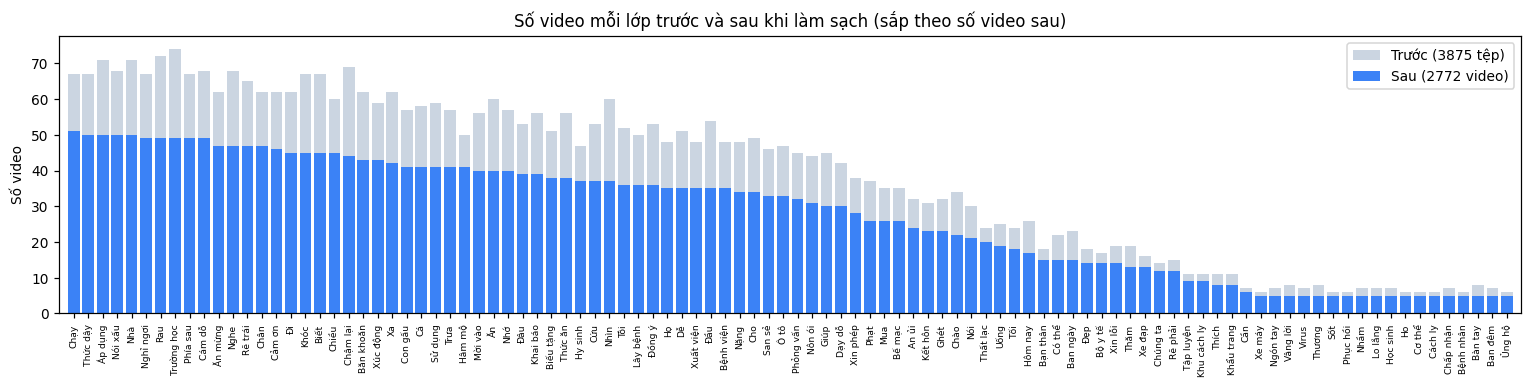
\includegraphics[width=\textwidth]{processing/class_counts_before_after.png}
  \caption{Số video mỗi lớp trước (xám) và sau (xanh) khi làm sạch, sắp xếp theo số video sau làm sạch.}
  \label{fig:pp_class_counts}
\end{figure}

% =====================================================================
\subsubsection{Xử lý khung nhiễu và lấy mẫu theo thời gian}
\label{subsec:pp_frames}

\paragraph{Bước 5 -- Đánh dấu khung đơn sắc} Gọi $f_i$ là khung thứ $i$ của video và $\sigma_c(f_i)$ là độ lệch chuẩn giá trị điểm ảnh trên kênh màu $c\in\{R,G,B\}$. Khung $f_i$ được coi là \emph{đơn sắc} nếu
\begin{equation}
  \max_{c\in\{R,G,B\}} \sigma_c(f_i) < 3,
\end{equation}
tức gần như mọi điểm ảnh có cùng một màu; ngưỡng này giống với ngưỡng ở bước EDA. Các khung còn lại là \emph{khung hợp lệ}. Thay vì xoá khung khỏi tệp video, notebook lưu danh sách chỉ số khung hợp lệ $V=(v_1<v_2<\dots<v_m)$ của từng video vào cột \texttt{valid\_idx} của manifest; khi đọc video, \texttt{preprocess.py} chỉ lấy mẫu trong danh sách này.

Trong 2.772 video sạch, 563 video (20,3\%, thuộc 78 lớp) có khung đơn sắc, trung bình 12,2 khung mỗi video. Sau khi bỏ khung đơn sắc, mỗi video còn từ 9 đến 30 khung hợp lệ (trung vị 30); 222 video còn ít hơn 16 khung hợp lệ (Hình~\ref{fig:pp_valid_hist}).

\begin{figure}[H]
  \centering
  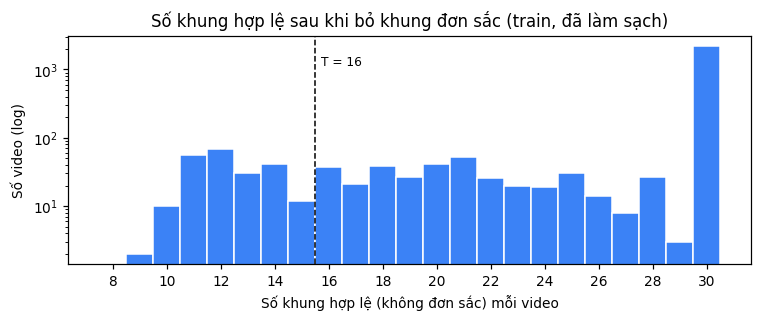
\includegraphics[width=0.75\textwidth]{processing/valid_frames_hist.png}
  \caption{Phân phối số khung hợp lệ mỗi video sau khi bỏ khung đơn sắc (trục tung thang log). Các video bên trái đường đứt nét có ít hơn $T=16$ khung hợp lệ.}
  \label{fig:pp_valid_hist}
\end{figure}

\paragraph{Bước 6 -- Lấy mẫu $T=16$ khung} Mô hình cần chuỗi đầu vào có độ dài cố định, nên mỗi video được thu gọn thành $T=16$ khung lấy đều theo thời gian trên danh sách khung hợp lệ:
\begin{equation}
  s_k = v_{\,1+\operatorname{round}\left(k\,\frac{m-1}{T-1}\right)}, \qquad k = 0, 1, \dots, T-1.
\end{equation}
Khung đầu và khung cuối của chuỗi luôn là khung hợp lệ đầu tiên và cuối cùng. Với video có $m<16$ khung hợp lệ, công thức trên tự lặp lại đều các khung (mỗi khung xuất hiện một hoặc hai lần) thay vì chỉ lặp khung cuối, nên chuỗi vẫn giữ đúng thứ tự thời gian. Nếu một video không có khung hợp lệ nào (chỉ có thể xảy ra ở dữ liệu kiểm tra hoặc demo) thì dùng toàn bộ khung.

Để thấy tác dụng của bước 5, nhóm so sánh với cách lấy mẫu đều trực tiếp trên toàn bộ khung, không lọc khung đơn sắc (Bảng~\ref{tab:pp_sampling}, Hình~\ref{fig:pp_sampling}). Nếu không lọc, cả 563 video có khung đơn sắc đều bị lẫn khung đơn sắc vào chuỗi đầu vào, trung bình 6,4/16 khung, và 222 video bị lẫn từ một nửa chuỗi trở lên; các số này khớp với mô phỏng ở bước EDA (Mục~\ref{subsec:eda_quality}). Khi lấy mẫu trên khung hợp lệ thì không còn khung đơn sắc nào trong đầu vào.

\begin{table}[H]
  \centering
  \caption{Số khung đơn sắc trong chuỗi 16 khung đầu vào, khi không lọc và khi lọc khung đơn sắc (2.772 video train sạch).}
  \label{tab:pp_sampling}
  \small
  \begin{tabular}{@{}lrr@{}}
    \toprule
    \textbf{Chỉ số} & \textbf{Không lọc} & \textbf{Có lọc} \\
    \midrule
    Video có $\geq$1 khung đơn sắc trong đầu vào   & 563 & 0 \\
    Số khung đơn sắc trung bình (trên các video đó) & 6,4/16 & 0 \\
    Video có $\geq$8/16 khung đơn sắc               & 222 & 0 \\
    \bottomrule
  \end{tabular}
\end{table}

\begin{figure}[H]
  \centering
  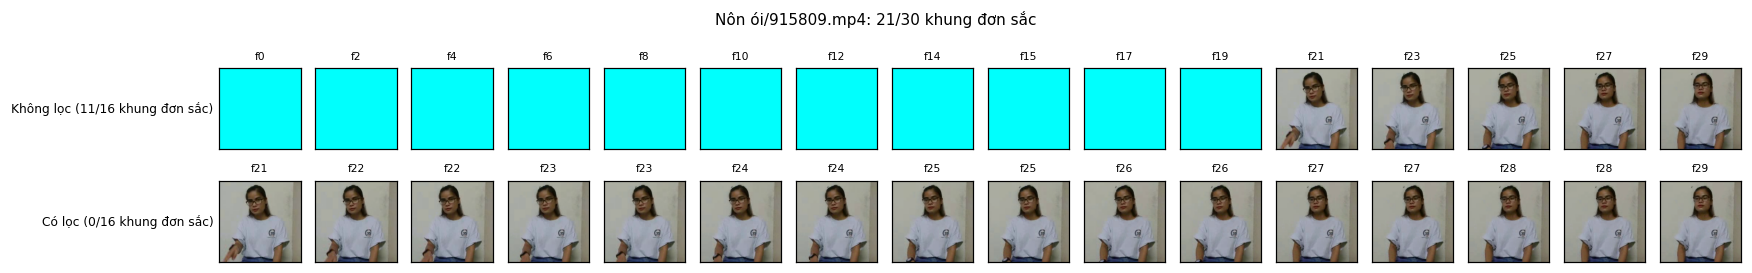
\includegraphics[width=\textwidth]{processing/sampling_naive_vs_filtered.png}
  \caption{Mười sáu khung đầu vào của video \textit{Nôn ói}/915809 (21/30 khung đơn sắc). Hàng trên: lấy mẫu trực tiếp, 11/16 khung là khung đơn sắc. Hàng dưới: lấy mẫu trên các khung hợp lệ $f_{21}$--$f_{29}$, các khung được lặp đều.}
  \label{fig:pp_sampling}
\end{figure}

% =====================================================================
\subsubsection{Chuẩn hoá}
\label{subsec:pp_norm}

\paragraph{Bước 7 -- Chuẩn hoá z-score} Giá trị điểm ảnh được đưa về $[0,1]$ rồi chuẩn hoá z-score trên từng kênh màu:
\begin{equation}
  x'_c = \frac{x_c/255 - \mu_c}{\sigma_c}, \qquad \mu = (0{,}485;\ 0{,}456;\ 0{,}406), \quad \sigma = (0{,}229;\ 0{,}224;\ 0{,}225),
\end{equation}
với $\mu,\sigma$ là trung bình và độ lệch chuẩn của tập ImageNet. Nhóm dùng thống kê của ImageNet thay vì tính lại trên tập train vì các mô hình ở Chương~\ref{sec:model} dùng mạng trích đặc trưng đã huấn luyện sẵn trên ImageNet; đầu vào cần có cùng phân phối với dữ liệu mà mạng đó đã học. Kết quả của mỗi video là một tensor kích thước $16\times3\times224\times224$. Độ phân giải đã đồng nhất $224\times224$ (Bảng~\ref{tab:eda_res}) nên không cần đổi kích thước.

% =====================================================================
\subsubsection{Chia tập huấn luyện và kiểm định}
\label{subsec:pp_split}

\paragraph{Bước 8 -- Chia phân tầng} Chỉ tập train có nhãn, nên tập kiểm định (\textit{validation}) phải tách ra từ chính tập này. Nhóm chia 2.772 video sạch thành 5 phần bằng \texttt{StratifiedKFold} của scikit-learn~\cite{sklearn} (\texttt{shuffle=True}, \texttt{random\_state=42}) và ghi số thứ tự phần vào cột \texttt{fold} của manifest. Phần \texttt{fold = 0} là tập kiểm định chung cho \emph{mọi} mô hình, các phần còn lại là tập huấn luyện; nhờ vậy kết quả của các mô hình so sánh được với nhau. Mô hình SVM có thể dùng cả 5 phần để kiểm định chéo (\textit{cross-validation}).

\begin{itemize}
  \item \textbf{Phân tầng theo nhãn:} mỗi phần giữ tỷ lệ các lớp gần giống toàn tập. Lớp nhỏ nhất có 5 video nên có đúng 1 video ở mỗi phần, nhờ đó cả 100 lớp đều có mặt ở tập kiểm định.
  \item \textbf{Không rò rỉ dữ liệu:} EDA khuyến nghị chia theo nhóm video gốc (\texttt{StratifiedGroupKFold}) để các bản sao không rơi vào cả hai phía. Vì bước 2 đã loại mọi bản sao, mỗi video sạch là một nhóm riêng, nên chia theo từng video cũng chính là chia theo nhóm. Notebook kiểm tra lại bằng \texttt{assert}: mã MD5 là duy nhất trong manifest và không có mã MD5 nào nằm ở cả tập huấn luyện lẫn tập kiểm định. Nhóm đã thử \texttt{StratifiedGroupKFold}, nhưng thuật toán này chỉ cân bằng gần đúng và tạo ra phần thiếu lớp.
\end{itemize}

\begin{table}[H]
  \centering
  \caption{Kết quả chia tập train sạch.}
  \label{tab:pp_split}
  \small
  \begin{tabular}{@{}lrrr@{}}
    \toprule
    \textbf{Tập} & \textbf{Số video} & \textbf{Số lớp} & \textbf{Số video mỗi lớp} \\
    \midrule
    Huấn luyện (\texttt{fold} 1--4) & 2.217 & 100 & 4--41 \\
    Kiểm định (\texttt{fold} 0)     & 555   & 100 & 1--10 \\
    \midrule
    Tổng                            & 2.772 & 100 & 5--51 \\
    \bottomrule
  \end{tabular}
\end{table}

% =====================================================================
\subsubsection{Xử lý mất cân bằng lớp}
\label{subsec:pp_weights}

\paragraph{Bước 9 -- Trọng số lớp} Trên tập huấn luyện, lớp nhiều nhất (\textit{Chạy}) có 41 video còn nhiều lớp chỉ có 4 video (\textit{Cách ly}, \textit{Ho}, \textit{Sốt}, \textit{Virus}, \textit{Xe máy},\ldots), chênh khoảng 10,2 lần. Nếu mọi mẫu có vai trò như nhau trong hàm mất mát, mô hình sẽ ưu tiên các lớp đông và Macro F1 giảm ở các lớp ít mẫu. Nhóm tính trọng số cho từng lớp $c$ theo kiểu \textit{balanced}:
\begin{equation}
  w_c = \frac{N}{K \cdot n_c},
\end{equation}
với $N=2.217$ là số video huấn luyện, $K=100$ là số lớp và $n_c$ là số video huấn luyện của lớp $c$. Lớp ít mẫu nhận trọng số lớn: trọng số dao động từ 0,54 (\textit{Chạy}) đến 5,54 (các lớp có 4 video), và một lớp trung bình ($n_c = N/K$) có trọng số bằng 1. Trọng số chỉ tính trên tập huấn luyện để không dùng thông tin của tập kiểm định. Các mô hình dùng trọng số này trong hàm mất mát (ví dụ tham số \texttt{weight} của \texttt{CrossEntropyLoss}) hoặc tham số \texttt{class\_weight} của SVM.

% =====================================================================
\subsubsection{Tăng cường dữ liệu}
\label{subsec:pp_aug}

\paragraph{Bước 10 -- Tăng cường} Tập huấn luyện nhỏ (trung bình khoảng 22 video mỗi lớp), nên mỗi lần đọc một video huấn luyện, \texttt{preprocess.py} tạo ra một biến thể ngẫu nhiên khác của video đó. Ba phép biến đổi được dùng, với cùng một tham số cho mọi khung của một video để chuyển động không bị méo:

\begin{itemize}
  \item \textbf{Cắt đoạn theo thời gian:} giữ một đoạn liên tục dài 80--100\% danh sách khung hợp lệ ở vị trí ngẫu nhiên, rồi mới lấy 16 khung. Phép này mô phỏng việc người ký bắt đầu, kết thúc sớm hay muộn và ký nhanh hay chậm khác nhau.
  \item \textbf{Cắt vùng ảnh ngẫu nhiên:} cắt một vùng có cạnh bằng 85--100\% cạnh khung hình ở vị trí ngẫu nhiên rồi phóng lại về $224\times224$. Phép này mô phỏng khác biệt về vị trí người ký và khoảng cách tới máy quay.
  \item \textbf{Thay đổi màu:} nhân độ sáng, độ tương phản và độ bão hoà với các hệ số ngẫu nhiên trong khoảng $[0{,}75;\ 1{,}25]$, giúp mô hình bền vững với khác biệt ánh sáng và màu nền giữa train và test (Mục~\ref{subsec:eda_shift}).
\end{itemize}

Nhóm \emph{không} dùng lật ngang vì tay trái và tay phải có thể làm đổi nghĩa ký hiệu. Tăng cường chỉ áp dụng cho tập huấn luyện; tập kiểm định và tập kiểm tra được đưa vào mô hình nguyên bản để kết quả đánh giá ổn định. Hình~\ref{fig:pp_aug} minh hoạ ba biến thể tạo ra từ cùng một video.

\begin{figure}[H]
  \centering
  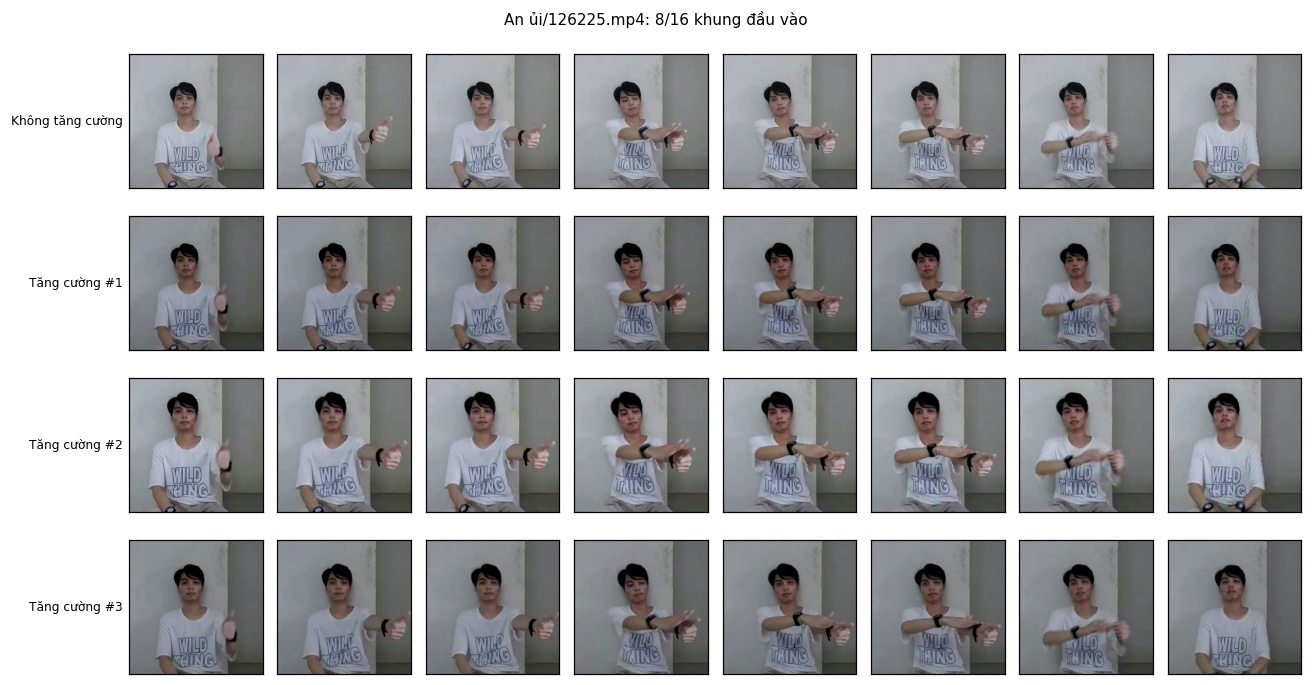
\includegraphics[width=0.9\textwidth]{processing/augmentation_examples.png}
  \caption{Một video lớp \textit{An ủi} (hàng đầu) và ba biến thể tăng cường ngẫu nhiên; mỗi hàng hiển thị 8 trong 16 khung đầu vào.}
  \label{fig:pp_aug}
\end{figure}

% =====================================================================
\subsubsection{Dữ liệu kiểm tra}
\label{subsec:pp_test}

Hai tập kiểm tra (\texttt{public\_test}, \texttt{private\_test}) không có nhãn và cuộc thi yêu cầu dự đoán cho \emph{mọi} tệp, nên nhóm không loại tệp nào. Notebook chỉ lập bảng \texttt{test\_manifest.csv} gồm tên tệp, mã MD5 và cột \texttt{dup\_of\_train} đánh dấu video trùng với tập train: có 157/1.630 video public test trùng với train và 0/2.859 video private test trùng với train. Các video trùng vẫn được mô hình dự đoán bình thường; cột này chỉ dùng khi diễn giải điểm public test (Mục~\ref{subsec:eda_quality}).

Khi suy luận, mỗi video kiểm tra đi qua đúng các bước 5, 6 và 7 như video kiểm định: tự tìm khung đơn sắc, lấy 16 khung trên các khung hợp lệ và chuẩn hoá, không tăng cường. Notebook chạy thử hàm đọc video này trên 8 video kiểm tra ngẫu nhiên để xác nhận đầu ra có đúng kích thước $16\times224\times224\times3$.

% =====================================================================
\subsubsection{Kết quả và đầu ra}
\label{subsec:pp_output}

Bảng~\ref{tab:pp_outputs} liệt kê các tệp do notebook tạo ra trong thư mục \texttt{processing/output/}. Các mô hình chỉ cần \texttt{preprocess.py}, \texttt{manifest\_clean.csv}, \texttt{test\_manifest.csv} và \texttt{class\_weights.csv} (vài trăm KB) cùng tệp dữ liệu gốc, không cần chạy lại bước làm sạch.

\begin{table}[H]
  \centering
  \caption{Các tệp đầu ra của bước tiền xử lý.}
  \label{tab:pp_outputs}
  \small
  \begin{tabular}{@{}p{0.3\textwidth}p{0.62\textwidth}@{}}
    \toprule
    \textbf{Tệp} & \textbf{Nội dung} \\
    \midrule
    \texttt{manifest\_clean.csv} & 2.772 video train sạch: lớp, nhãn số, tên tệp, đường dẫn, MD5, số khung, số khung hợp lệ, chỉ số khung hợp lệ (\texttt{valid\_idx}), phần (\texttt{fold}) \\
    \texttt{removed.csv} & 1.103 tệp bị loại, kèm bước và lý do \\
    \texttt{test\_manifest.csv} & 4.489 video kiểm tra: tập, tên tệp, MD5, \texttt{dup\_of\_train} \\
    \texttt{class\_weights.csv} & Trọng số 100 lớp tính trên tập huấn luyện \\
    \texttt{processing\_summary.csv} & Số video còn lại sau từng bước (Bảng~\ref{tab:pp_flow}) \\
    \texttt{class\_counts\_before\_after.csv} & Số video mỗi lớp trước và sau làm sạch \\
    \texttt{processing\_config.json} & Tham số đã dùng (\texttt{SEED}, số phần, $T$, ngưỡng đơn sắc) \\
    \texttt{figures/} & Các hình trong mục này \\
    \bottomrule
  \end{tabular}
\end{table}

Tóm lại, sau tiền xử lý tập train không còn bản sao, video rỗng hay nhãn mâu thuẫn; không video nào còn khung đơn sắc trong chuỗi đầu vào; tập kiểm định đủ 100 lớp và không chứa video trùng với tập huấn luyện. Các bước này xử lý cả ba vấn đề chính mà EDA đã nêu: bản sao gây rò rỉ dữ liệu, khung đơn sắc chỉ có ở train và mất cân bằng lớp.

\paragraph{Hạn chế} Nhóm chưa xác định được nhãn đúng cho hai nội dung xung đột nên phải bỏ chúng, làm giảm 5 tệp dữ liệu có thể hữu ích. Ngưỡng đơn sắc chỉ phát hiện khung một màu hoàn toàn, chưa phát hiện khung mờ hoặc khung chỉ có nền. Khử trùng lặp bằng MD5 chỉ tìm được bản sao giống hệt từng byte, không tìm được video gần giống nhau (ví dụ cùng cảnh nhưng nén lại). Cuối cùng, tập kiểm định chỉ có 1--10 video mỗi lớp, nên F1 của từng lớp riêng lẻ trên tập này còn dao động lớn.
]
% Mã nguồn: processing/data_processing.ipynb, processing/preprocess.py
% Hình: image/processing/*.png (sinh từ processing/output/figures/)
%   3.2.1 Tổng quan quy trình
%   3.2.2 Làm sạch dữ liệu
%   3.2.3 Xử lý khung nhiễu và lấy mẫu theo thời gian
%   3.2.4 Chuẩn hoá
%   3.2.5 Chia tập huấn luyện và kiểm định
%   3.2.6 Xử lý mất cân bằng lớp
%   3.2.7 Tăng cường dữ liệu
%   3.2.8 Dữ liệu kiểm tra
%   3.2.9 Kết quả và đầu ra
% =====================================================================

\subsection{Tiền xử lý dữ liệu}
\label{sec:preprocess}

Mục này trình bày các bước biến dữ liệu thô thành đầu vào sạch và thống nhất cho mọi mô hình ở Chương~\ref{sec:model}. Mỗi bước xuất phát từ một vấn đề đã phát hiện ở bước EDA (Bảng~\ref{tab:eda_reco}). Nhóm dùng Python với \texttt{pandas}, \texttt{numpy}, \texttt{OpenCV} và \texttt{scikit-learn}; mã nguồn gồm hai phần:

\begin{itemize}
  \item \textbf{Notebook làm sạch} \texttt{processing/data\_processing.ipynb}: chạy \emph{một lần} trên toàn bộ tập train để kiểm tra, loại bỏ và đánh dấu dữ liệu lỗi, chia tập kiểm định và tính trọng số lớp. Kết quả được lưu thành một bảng chỉ mục (\textit{manifest}) dùng chung cho cả nhóm.
  \item \textbf{Module dùng chung} \texttt{processing/preprocess.py}: các phép biến đổi áp dụng \emph{mỗi lần} mô hình đọc một video (bỏ khung đơn sắc, lấy mẫu khung, tăng cường, chuẩn hoá). Mô hình SVM, CNN-LSTM, Vision Transformer và ứng dụng demo cùng gọi module này, nên dữ liệu ở huấn luyện, kiểm định, kiểm tra và demo được xử lý giống hệt nhau.
\end{itemize}

Nhóm không lưu sẵn khung hình đã xử lý ra đĩa vì hai lý do: lưu 16 khung $224\times224\times3$ cho 2.772 video tốn khoảng 6,7~GB, và phép tăng cường cần tạo ra phiên bản khác nhau ở mỗi lần đọc. Mọi bước có yếu tố ngẫu nhiên đều cố định hạt giống \texttt{SEED = 42} để kết quả tái lập được.

% =====================================================================
\subsubsection{Tổng quan quy trình}
\label{subsec:pp_overview}

Bảng~\ref{tab:pp_overview} liệt kê mười bước tiền xử lý theo thứ tự thực hiện và xếp mỗi bước vào nhóm tác vụ tiền xử lý dữ liệu tương ứng: làm sạch (\textit{data cleaning}), tích hợp (\textit{data integration}), thu gọn (\textit{data reduction}) và biến đổi dữ liệu (\textit{data transformation})~\cite{han2011}.

\begin{table}[H]
  \centering
  \caption{Các bước tiền xử lý, nhóm tác vụ và nơi thực hiện.}
  \label{tab:pp_overview}
  \small
  \begin{tabular}{@{}cp{0.33\textwidth}p{0.3\textwidth}p{0.2\textwidth}@{}}
    \toprule
    \textbf{Bước} & \textbf{Việc} & \textbf{Nhóm tác vụ} & \textbf{Thực hiện ở} \\
    \midrule
    1  & Kiểm tra toàn vẹn, chuẩn hoá tên lớp & Làm sạch: dữ liệu thiếu, lỗi & Notebook \\
    2  & Khử trùng lặp theo MD5 & Tích hợp: dư thừa dữ liệu & Notebook \\
    3  & Loại video xung đột nhãn & Làm sạch: dữ liệu không nhất quán & Notebook \\
    4  & Loại video rỗng & Làm sạch: dữ liệu thiếu & Notebook \\
    5  & Đánh dấu khung đơn sắc & Làm sạch: dữ liệu nhiễu & Notebook, \texttt{preprocess.py} \\
    6  & Lấy đều $T=16$ khung trên các khung hợp lệ & Thu gọn: lấy mẫu & \texttt{preprocess.py} \\
    7  & Chuẩn hoá z-score theo kênh màu & Biến đổi: chuẩn hoá & \texttt{preprocess.py} \\
    8  & Chia train/validation phân tầng & Đánh giá mô hình & Notebook \\
    9  & Trọng số lớp & Xử lý mất cân bằng lớp & Notebook \\
    10 & Tăng cường dữ liệu (chỉ khi huấn luyện) & Sinh thêm dữ liệu & \texttt{preprocess.py} \\
    \bottomrule
  \end{tabular}
\end{table}

Bước 1--5 thu hẹp tập train từ 3.875 tệp xuống 2.772 video sạch (Bảng~\ref{tab:pp_flow}). Bước 6, 7 và 10 không bỏ video nào mà quyết định video được đưa vào mô hình dưới dạng nào. Bước 8 và 9 chuẩn bị cho huấn luyện và đánh giá.

% =====================================================================
\subsubsection{Làm sạch dữ liệu}
\label{subsec:pp_clean}

\paragraph{Quét toàn bộ video} Notebook mở từng video bằng \texttt{cv2.VideoCapture}, đọc \emph{tất cả} khung hình và ghi lại: mã băm MD5 của tệp, số khung, và danh sách chỉ số các khung không đơn sắc (Mục~\ref{subsec:pp_frames}). Việc quét được chạy song song trên nhiều lõi CPU (\texttt{ProcessPoolExecutor}). Để kiểm tra bước quét, nhóm đối chiếu số khung đơn sắc của từng video với cột \texttt{solid\_frames} trong \texttt{video\_quality\_flags.csv} của bước EDA: cả 3.875/3.875 tệp đều khớp.

\paragraph{Bước 1 -- Kiểm tra toàn vẹn} Cả 3.875 tệp đều đọc được và có ít nhất 16 khung, nên không có tệp nào bị loại ở bước này. Tên lớp ở thư mục và khoá trong \texttt{label\_mapping.pkl} được chuẩn hoá về dạng Unicode NFC trước khi so khớp (Mục~\ref{subsec:eda_structure}); sau chuẩn hoá, 100/100 lớp có nhãn số 0--99.

\paragraph{Bước 2 -- Khử trùng lặp} Hai tệp có cùng mã MD5 là cùng một video. Với mỗi mã MD5, notebook giữ lại một tệp (ưu tiên tệp không có hậu tố \texttt{\_N}) và loại các tệp còn lại. Bước này loại 1.099 tệp, trong đó 1.069 tệp mang hậu tố \texttt{\_N}, và còn \textbf{2.776 video duy nhất}, khớp với kết quả EDA. Từ đây mỗi video trong tập sạch có một mã MD5 riêng; tính chất này giúp chia tập kiểm định không bị rò rỉ (Mục~\ref{subsec:pp_split}).

\paragraph{Bước 3 -- Xung đột nhãn} Hai nội dung video vừa nằm ở lớp \textit{Chào} vừa nằm ở lớp \textit{Chậm lại} (5 tệp: \texttt{Chào/392683}, \texttt{Chào/468203}, \texttt{Chào/792094}, \texttt{Chậm lại/254739}, \texttt{Chậm lại/284430}). Nhóm không xác minh được nhãn nào đúng, và giữ một video với nhãn có thể sai sẽ đưa nhiễu nhãn vào cả huấn luyện lẫn đánh giá, nên loại toàn bộ hai nội dung này. Notebook có sẵn biến \texttt{KEEP\_LABEL} để giữ lại các video này với nhãn đã xác minh nếu sau này có thông tin. Sau bước này còn 2.774 video. Hai lớp bị ảnh hưởng vẫn còn nhiều mẫu (\textit{Chào} 22 video, \textit{Chậm lại} 44 video).

\paragraph{Bước 4 -- Video rỗng} Hai video không có khung hợp lệ nào (\texttt{Biết/214576}: 16/16 khung đơn sắc; \texttt{Khai báo/885339}: 23/23 khung đơn sắc) bị loại vì không chứa thông tin ký hiệu. Tập train sạch còn \textbf{2.772 video} và vẫn đủ 100 lớp.

\begin{table}[H]
  \centering
  \caption{Số video còn lại sau từng bước làm sạch tập train.}
  \label{tab:pp_flow}
  \small
  \begin{tabular}{@{}p{0.3\textwidth}rp{0.45\textwidth}@{}}
    \toprule
    \textbf{Bước} & \textbf{Còn lại} & \textbf{Ghi chú} \\
    \midrule
    Ban đầu                          & 3.875 & Toàn bộ tệp trong \texttt{train/} \\
    1 -- Kiểm tra toàn vẹn           & 3.875 & Không có tệp lỗi hoặc thiếu khung \\
    2 -- Khử trùng lặp MD5           & 2.776 & Loại 1.099 bản sao \\
    3 -- Xung đột nhãn               & 2.774 & Loại 2 nội dung (5 tệp) \textit{Chào} $\leftrightarrow$ \textit{Chậm lại} \\
    4 -- Video rỗng                  & \textbf{2.772} & Loại \texttt{Biết/214576}, \texttt{Khai báo/885339} \\
    5 -- Khung đơn sắc               & 2.772 & 563 video có khung bị bỏ qua, không loại video \\
    \bottomrule
  \end{tabular}
\end{table}

Danh sách 1.103 tệp bị loại cùng lý do được lưu ở \texttt{processing/output/removed.csv}, để có thể kiểm tra lại từng trường hợp. Hình~\ref{fig:pp_class_counts} so sánh số video mỗi lớp trước và sau khi làm sạch: sau làm sạch mỗi lớp có từ 5 đến 51 video (trung bình 27,7; trung vị 32,5).

\begin{figure}[H]
  \centering
  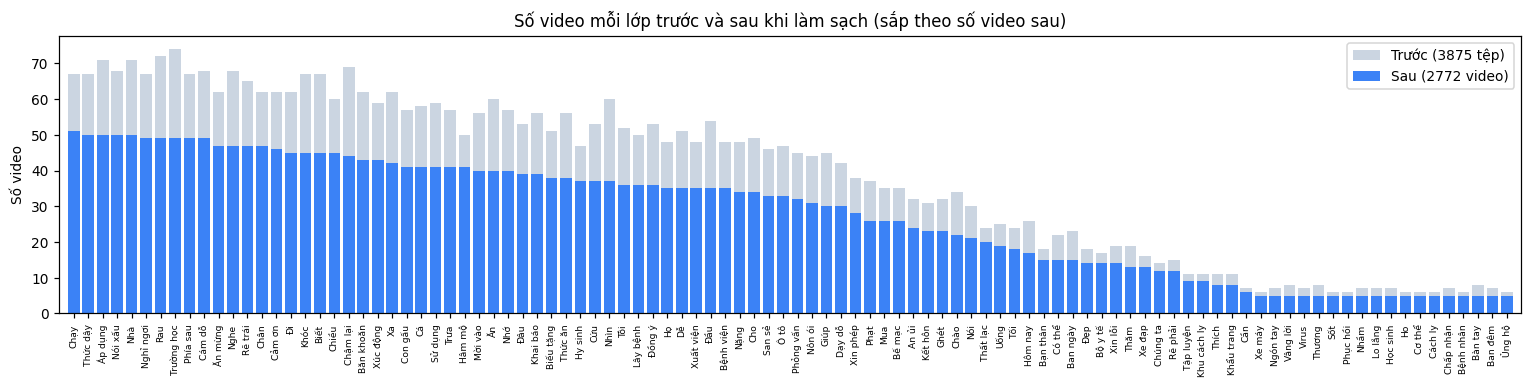
\includegraphics[width=\textwidth]{processing/class_counts_before_after.png}
  \caption{Số video mỗi lớp trước (xám) và sau (xanh) khi làm sạch, sắp xếp theo số video sau làm sạch.}
  \label{fig:pp_class_counts}
\end{figure}

% =====================================================================
\subsubsection{Xử lý khung nhiễu và lấy mẫu theo thời gian}
\label{subsec:pp_frames}

\paragraph{Bước 5 -- Đánh dấu khung đơn sắc} Gọi $f_i$ là khung thứ $i$ của video và $\sigma_c(f_i)$ là độ lệch chuẩn giá trị điểm ảnh trên kênh màu $c\in\{R,G,B\}$. Khung $f_i$ được coi là \emph{đơn sắc} nếu
\begin{equation}
  \max_{c\in\{R,G,B\}} \sigma_c(f_i) < 3,
\end{equation}
tức gần như mọi điểm ảnh có cùng một màu; ngưỡng này giống với ngưỡng ở bước EDA. Các khung còn lại là \emph{khung hợp lệ}. Thay vì xoá khung khỏi tệp video, notebook lưu danh sách chỉ số khung hợp lệ $V=(v_1<v_2<\dots<v_m)$ của từng video vào cột \texttt{valid\_idx} của manifest; khi đọc video, \texttt{preprocess.py} chỉ lấy mẫu trong danh sách này.

Trong 2.772 video sạch, 563 video (20,3\%, thuộc 78 lớp) có khung đơn sắc, trung bình 12,2 khung mỗi video. Sau khi bỏ khung đơn sắc, mỗi video còn từ 9 đến 30 khung hợp lệ (trung vị 30); 222 video còn ít hơn 16 khung hợp lệ (Hình~\ref{fig:pp_valid_hist}).

\begin{figure}[H]
  \centering
  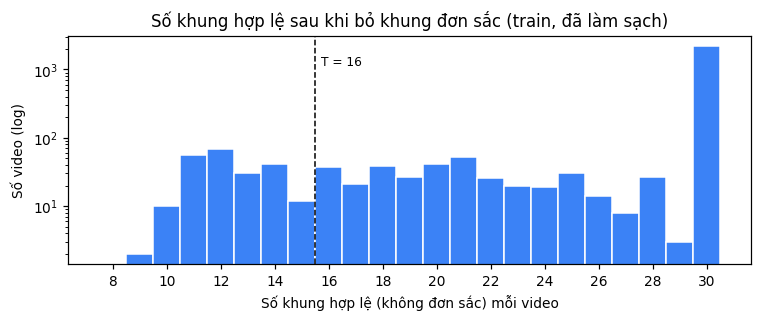
\includegraphics[width=0.75\textwidth]{processing/valid_frames_hist.png}
  \caption{Phân phối số khung hợp lệ mỗi video sau khi bỏ khung đơn sắc (trục tung thang log). Các video bên trái đường đứt nét có ít hơn $T=16$ khung hợp lệ.}
  \label{fig:pp_valid_hist}
\end{figure}

\paragraph{Bước 6 -- Lấy mẫu $T=16$ khung} Mô hình cần chuỗi đầu vào có độ dài cố định, nên mỗi video được thu gọn thành $T=16$ khung lấy đều theo thời gian trên danh sách khung hợp lệ:
\begin{equation}
  s_k = v_{\,1+\operatorname{round}\left(k\,\frac{m-1}{T-1}\right)}, \qquad k = 0, 1, \dots, T-1.
\end{equation}
Khung đầu và khung cuối của chuỗi luôn là khung hợp lệ đầu tiên và cuối cùng. Với video có $m<16$ khung hợp lệ, công thức trên tự lặp lại đều các khung (mỗi khung xuất hiện một hoặc hai lần) thay vì chỉ lặp khung cuối, nên chuỗi vẫn giữ đúng thứ tự thời gian. Nếu một video không có khung hợp lệ nào (chỉ có thể xảy ra ở dữ liệu kiểm tra hoặc demo) thì dùng toàn bộ khung.

Để thấy tác dụng của bước 5, nhóm so sánh với cách lấy mẫu đều trực tiếp trên toàn bộ khung, không lọc khung đơn sắc (Bảng~\ref{tab:pp_sampling}, Hình~\ref{fig:pp_sampling}). Nếu không lọc, cả 563 video có khung đơn sắc đều bị lẫn khung đơn sắc vào chuỗi đầu vào, trung bình 6,4/16 khung, và 222 video bị lẫn từ một nửa chuỗi trở lên; các số này khớp với mô phỏng ở bước EDA (Mục~\ref{subsec:eda_quality}). Khi lấy mẫu trên khung hợp lệ thì không còn khung đơn sắc nào trong đầu vào.

\begin{table}[H]
  \centering
  \caption{Số khung đơn sắc trong chuỗi 16 khung đầu vào, khi không lọc và khi lọc khung đơn sắc (2.772 video train sạch).}
  \label{tab:pp_sampling}
  \small
  \begin{tabular}{@{}lrr@{}}
    \toprule
    \textbf{Chỉ số} & \textbf{Không lọc} & \textbf{Có lọc} \\
    \midrule
    Video có $\geq$1 khung đơn sắc trong đầu vào   & 563 & 0 \\
    Số khung đơn sắc trung bình (trên các video đó) & 6,4/16 & 0 \\
    Video có $\geq$8/16 khung đơn sắc               & 222 & 0 \\
    \bottomrule
  \end{tabular}
\end{table}

\begin{figure}[H]
  \centering
  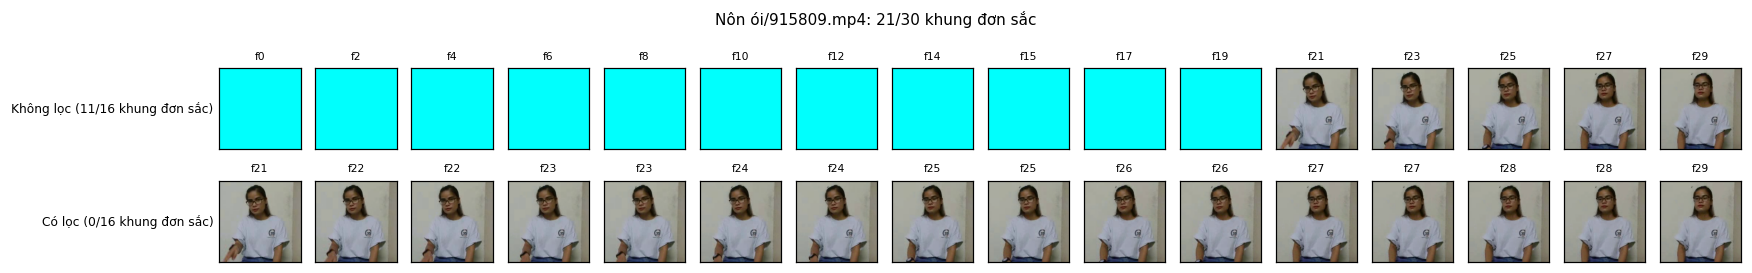
\includegraphics[width=\textwidth]{processing/sampling_naive_vs_filtered.png}
  \caption{Mười sáu khung đầu vào của video \textit{Nôn ói}/915809 (21/30 khung đơn sắc). Hàng trên: lấy mẫu trực tiếp, 11/16 khung là khung đơn sắc. Hàng dưới: lấy mẫu trên các khung hợp lệ $f_{21}$--$f_{29}$, các khung được lặp đều.}
  \label{fig:pp_sampling}
\end{figure}

% =====================================================================
\subsubsection{Chuẩn hoá}
\label{subsec:pp_norm}

\paragraph{Bước 7 -- Chuẩn hoá z-score} Giá trị điểm ảnh được đưa về $[0,1]$ rồi chuẩn hoá z-score trên từng kênh màu:
\begin{equation}
  x'_c = \frac{x_c/255 - \mu_c}{\sigma_c}, \qquad \mu = (0{,}485;\ 0{,}456;\ 0{,}406), \quad \sigma = (0{,}229;\ 0{,}224;\ 0{,}225),
\end{equation}
với $\mu,\sigma$ là trung bình và độ lệch chuẩn của tập ImageNet. Nhóm dùng thống kê của ImageNet thay vì tính lại trên tập train vì các mô hình ở Chương~\ref{sec:model} dùng mạng trích đặc trưng đã huấn luyện sẵn trên ImageNet; đầu vào cần có cùng phân phối với dữ liệu mà mạng đó đã học. Kết quả của mỗi video là một tensor kích thước $16\times3\times224\times224$. Độ phân giải đã đồng nhất $224\times224$ (Bảng~\ref{tab:eda_res}) nên không cần đổi kích thước.

% =====================================================================
\subsubsection{Chia tập huấn luyện và kiểm định}
\label{subsec:pp_split}

\paragraph{Bước 8 -- Chia phân tầng} Chỉ tập train có nhãn, nên tập kiểm định (\textit{validation}) phải tách ra từ chính tập này. Nhóm chia 2.772 video sạch thành 5 phần bằng \texttt{StratifiedKFold} của scikit-learn~\cite{sklearn} (\texttt{shuffle=True}, \texttt{random\_state=42}) và ghi số thứ tự phần vào cột \texttt{fold} của manifest. Phần \texttt{fold = 0} là tập kiểm định chung cho \emph{mọi} mô hình, các phần còn lại là tập huấn luyện; nhờ vậy kết quả của các mô hình so sánh được với nhau. Mô hình SVM có thể dùng cả 5 phần để kiểm định chéo (\textit{cross-validation}).

\begin{itemize}
  \item \textbf{Phân tầng theo nhãn:} mỗi phần giữ tỷ lệ các lớp gần giống toàn tập. Lớp nhỏ nhất có 5 video nên có đúng 1 video ở mỗi phần, nhờ đó cả 100 lớp đều có mặt ở tập kiểm định.
  \item \textbf{Không rò rỉ dữ liệu:} EDA khuyến nghị chia theo nhóm video gốc (\texttt{StratifiedGroupKFold}) để các bản sao không rơi vào cả hai phía. Vì bước 2 đã loại mọi bản sao, mỗi video sạch là một nhóm riêng, nên chia theo từng video cũng chính là chia theo nhóm. Notebook kiểm tra lại bằng \texttt{assert}: mã MD5 là duy nhất trong manifest và không có mã MD5 nào nằm ở cả tập huấn luyện lẫn tập kiểm định. Nhóm đã thử \texttt{StratifiedGroupKFold}, nhưng thuật toán này chỉ cân bằng gần đúng và tạo ra phần thiếu lớp.
\end{itemize}

\begin{table}[H]
  \centering
  \caption{Kết quả chia tập train sạch.}
  \label{tab:pp_split}
  \small
  \begin{tabular}{@{}lrrr@{}}
    \toprule
    \textbf{Tập} & \textbf{Số video} & \textbf{Số lớp} & \textbf{Số video mỗi lớp} \\
    \midrule
    Huấn luyện (\texttt{fold} 1--4) & 2.217 & 100 & 4--41 \\
    Kiểm định (\texttt{fold} 0)     & 555   & 100 & 1--10 \\
    \midrule
    Tổng                            & 2.772 & 100 & 5--51 \\
    \bottomrule
  \end{tabular}
\end{table}

% =====================================================================
\subsubsection{Xử lý mất cân bằng lớp}
\label{subsec:pp_weights}

\paragraph{Bước 9 -- Trọng số lớp} Trên tập huấn luyện, lớp nhiều nhất (\textit{Chạy}) có 41 video còn nhiều lớp chỉ có 4 video (\textit{Cách ly}, \textit{Ho}, \textit{Sốt}, \textit{Virus}, \textit{Xe máy},\ldots), chênh khoảng 10,2 lần. Nếu mọi mẫu có vai trò như nhau trong hàm mất mát, mô hình sẽ ưu tiên các lớp đông và Macro F1 giảm ở các lớp ít mẫu. Nhóm tính trọng số cho từng lớp $c$ theo kiểu \textit{balanced}:
\begin{equation}
  w_c = \frac{N}{K \cdot n_c},
\end{equation}
với $N=2.217$ là số video huấn luyện, $K=100$ là số lớp và $n_c$ là số video huấn luyện của lớp $c$. Lớp ít mẫu nhận trọng số lớn: trọng số dao động từ 0,54 (\textit{Chạy}) đến 5,54 (các lớp có 4 video), và một lớp trung bình ($n_c = N/K$) có trọng số bằng 1. Trọng số chỉ tính trên tập huấn luyện để không dùng thông tin của tập kiểm định. Các mô hình dùng trọng số này trong hàm mất mát (ví dụ tham số \texttt{weight} của \texttt{CrossEntropyLoss}) hoặc tham số \texttt{class\_weight} của SVM.

% =====================================================================
\subsubsection{Tăng cường dữ liệu}
\label{subsec:pp_aug}

\paragraph{Bước 10 -- Tăng cường} Tập huấn luyện nhỏ (trung bình khoảng 22 video mỗi lớp), nên mỗi lần đọc một video huấn luyện, \texttt{preprocess.py} tạo ra một biến thể ngẫu nhiên khác của video đó. Ba phép biến đổi được dùng, với cùng một tham số cho mọi khung của một video để chuyển động không bị méo:

\begin{itemize}
  \item \textbf{Cắt đoạn theo thời gian:} giữ một đoạn liên tục dài 80--100\% danh sách khung hợp lệ ở vị trí ngẫu nhiên, rồi mới lấy 16 khung. Phép này mô phỏng việc người ký bắt đầu, kết thúc sớm hay muộn và ký nhanh hay chậm khác nhau.
  \item \textbf{Cắt vùng ảnh ngẫu nhiên:} cắt một vùng có cạnh bằng 85--100\% cạnh khung hình ở vị trí ngẫu nhiên rồi phóng lại về $224\times224$. Phép này mô phỏng khác biệt về vị trí người ký và khoảng cách tới máy quay.
  \item \textbf{Thay đổi màu:} nhân độ sáng, độ tương phản và độ bão hoà với các hệ số ngẫu nhiên trong khoảng $[0{,}75;\ 1{,}25]$, giúp mô hình bền vững với khác biệt ánh sáng và màu nền giữa train và test (Mục~\ref{subsec:eda_shift}).
\end{itemize}

Nhóm \emph{không} dùng lật ngang vì tay trái và tay phải có thể làm đổi nghĩa ký hiệu. Tăng cường chỉ áp dụng cho tập huấn luyện; tập kiểm định và tập kiểm tra được đưa vào mô hình nguyên bản để kết quả đánh giá ổn định. Hình~\ref{fig:pp_aug} minh hoạ ba biến thể tạo ra từ cùng một video.

\begin{figure}[H]
  \centering
  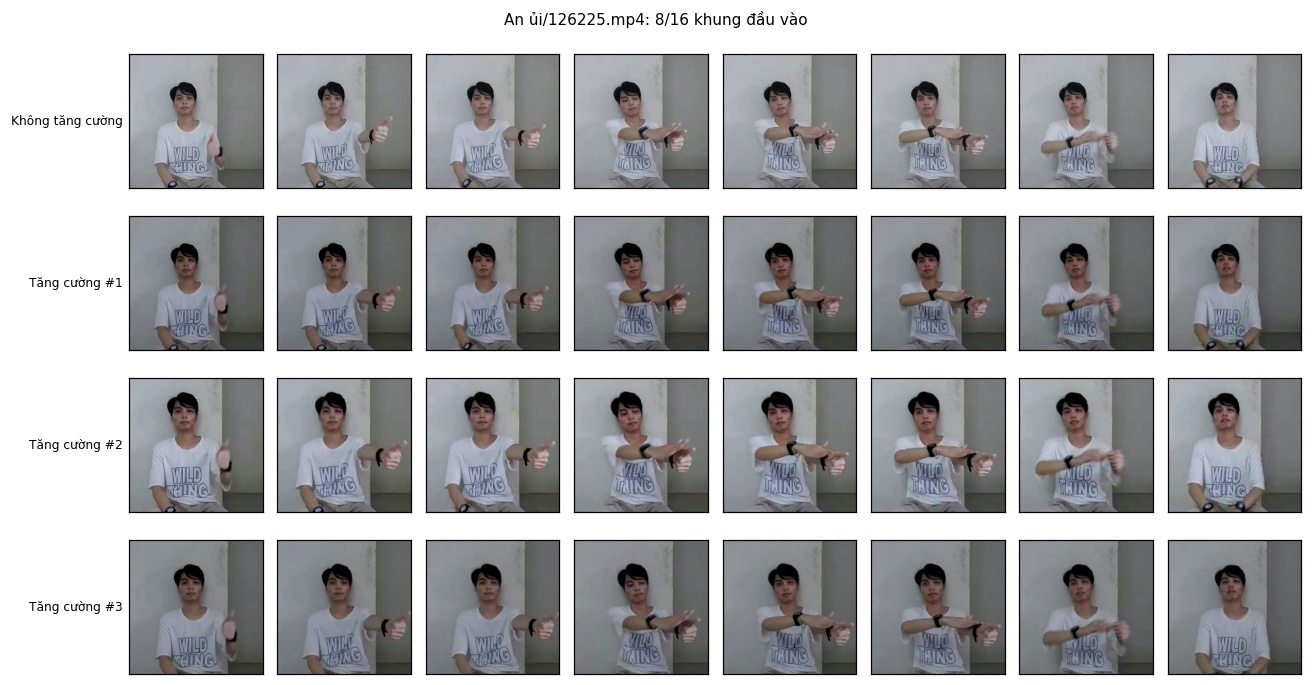
\includegraphics[width=0.9\textwidth]{processing/augmentation_examples.png}
  \caption{Một video lớp \textit{An ủi} (hàng đầu) và ba biến thể tăng cường ngẫu nhiên; mỗi hàng hiển thị 8 trong 16 khung đầu vào.}
  \label{fig:pp_aug}
\end{figure}

% =====================================================================
\subsubsection{Dữ liệu kiểm tra}
\label{subsec:pp_test}

Hai tập kiểm tra (\texttt{public\_test}, \texttt{private\_test}) không có nhãn và cuộc thi yêu cầu dự đoán cho \emph{mọi} tệp, nên nhóm không loại tệp nào. Notebook chỉ lập bảng \texttt{test\_manifest.csv} gồm tên tệp, mã MD5 và cột \texttt{dup\_of\_train} đánh dấu video trùng với tập train: có 157/1.630 video public test trùng với train và 0/2.859 video private test trùng với train. Các video trùng vẫn được mô hình dự đoán bình thường; cột này chỉ dùng khi diễn giải điểm public test (Mục~\ref{subsec:eda_quality}).

Khi suy luận, mỗi video kiểm tra đi qua đúng các bước 5, 6 và 7 như video kiểm định: tự tìm khung đơn sắc, lấy 16 khung trên các khung hợp lệ và chuẩn hoá, không tăng cường. Notebook chạy thử hàm đọc video này trên 8 video kiểm tra ngẫu nhiên để xác nhận đầu ra có đúng kích thước $16\times224\times224\times3$.

% =====================================================================
\subsubsection{Kết quả và đầu ra}
\label{subsec:pp_output}

Bảng~\ref{tab:pp_outputs} liệt kê các tệp do notebook tạo ra trong thư mục \texttt{processing/output/}. Các mô hình chỉ cần \texttt{preprocess.py}, \texttt{manifest\_clean.csv}, \texttt{test\_manifest.csv} và \texttt{class\_weights.csv} (vài trăm KB) cùng tệp dữ liệu gốc, không cần chạy lại bước làm sạch.

\begin{table}[H]
  \centering
  \caption{Các tệp đầu ra của bước tiền xử lý.}
  \label{tab:pp_outputs}
  \small
  \begin{tabular}{@{}p{0.3\textwidth}p{0.62\textwidth}@{}}
    \toprule
    \textbf{Tệp} & \textbf{Nội dung} \\
    \midrule
    \texttt{manifest\_clean.csv} & 2.772 video train sạch: lớp, nhãn số, tên tệp, đường dẫn, MD5, số khung, số khung hợp lệ, chỉ số khung hợp lệ (\texttt{valid\_idx}), phần (\texttt{fold}) \\
    \texttt{removed.csv} & 1.103 tệp bị loại, kèm bước và lý do \\
    \texttt{test\_manifest.csv} & 4.489 video kiểm tra: tập, tên tệp, MD5, \texttt{dup\_of\_train} \\
    \texttt{class\_weights.csv} & Trọng số 100 lớp tính trên tập huấn luyện \\
    \texttt{processing\_summary.csv} & Số video còn lại sau từng bước (Bảng~\ref{tab:pp_flow}) \\
    \texttt{class\_counts\_before\_after.csv} & Số video mỗi lớp trước và sau làm sạch \\
    \texttt{processing\_config.json} & Tham số đã dùng (\texttt{SEED}, số phần, $T$, ngưỡng đơn sắc) \\
    \texttt{figures/} & Các hình trong mục này \\
    \bottomrule
  \end{tabular}
\end{table}

Tóm lại, sau tiền xử lý tập train không còn bản sao, video rỗng hay nhãn mâu thuẫn; không video nào còn khung đơn sắc trong chuỗi đầu vào; tập kiểm định đủ 100 lớp và không chứa video trùng với tập huấn luyện. Các bước này xử lý cả ba vấn đề chính mà EDA đã nêu: bản sao gây rò rỉ dữ liệu, khung đơn sắc chỉ có ở train và mất cân bằng lớp.

\paragraph{Hạn chế} Nhóm chưa xác định được nhãn đúng cho hai nội dung xung đột nên phải bỏ chúng, làm giảm 5 tệp dữ liệu có thể hữu ích. Ngưỡng đơn sắc chỉ phát hiện khung một màu hoàn toàn, chưa phát hiện khung mờ hoặc khung chỉ có nền. Khử trùng lặp bằng MD5 chỉ tìm được bản sao giống hệt từng byte, không tìm được video gần giống nhau (ví dụ cùng cảnh nhưng nén lại). Cuối cùng, tập kiểm định chỉ có 1--10 video mỗi lớp, nên F1 của từng lớp riêng lẻ trên tập này còn dao động lớn.
